\documentclass[10pt,aspectratio=169,dvipsnames]{beamer}
\usetheme[]{Berlin}

\setbeamertemplate{footline}{
  \usebeamercolor[fg]{framesource}%
  \usebeamerfont{page number in head}%
  \hspace{0.2cm}
  \small \insertframenumber
  \vspace{0.2cm}
  \doclicenseIcon
  \hfill
  
\includegraphics[height=0.8cm]{logos/tub_logo.pdf}
  \hspace{0.2cm}
}

\setbeamercovered{transparent}

\setbeamertemplate{footline}[
 myframe number]

% PACKAGES
\usepackage[absolute,overlay]{textpos}
\usepackage[utf8]{inputenc}
\usepackage[official]{eurosym}
\usepackage{booktabs,multicol,multirow,tabularx,array}
\usepackage{subcaption}
\usepackage{parskip}
\usepackage{bm}
\usepackage{tikz}
\usepackage{adjustbox}
\usepackage[super]{nth}
\usepackage[version=4]{mhchem}
\usepackage{siunitx}
\sisetup{
  detect-all = true
}


\usepackage[
    type={CC},
    modifier={by},
    version={4.0},
]{doclicense}

% HYPERREFERENCES
\usepackage{hyperref}
\hypersetup{
	colorlinks=true,
	citecolor=tub-blue,
	linkcolor=tub-blue,
	urlcolor=tub-blue
}

\usepackage[sfdefault]{roboto}
\usepackage[normalem]{ulem}

\usepackage[backend=biber,style=numeric-comp]{biblatex}
\addbibresource{references.bib}

\newcolumntype{R}[1]{>{\raggedleft\arraybackslash}p{#1}}


% GRAPHICS	
\graphicspath{
    {graphics/},
    {../../../paper/first-draft/figures} % study results
  }
\DeclareGraphicsExtensions{.pdf,.jpeg,.png,.jpg}

% FORMATTING
\setlength{\parskip}{6pt}
\linespread{1.1}
\newcommand{\seprule}{\par\noindent\textcolor{black!25}{\rule{\textwidth}{0.4pt}}}

% SOURCES
\setbeamercolor{framesource}{fg=gray}
\setbeamerfont{framesource}{size=\tiny}
\newcommand{\source}[1]{\begin{textblock*}{10cm}(3.6cm,8.25cm)
    \begin{beamercolorbox}[ht=0.5cm,right]{framesource}
        \usebeamerfont{framesource}\usebeamercolor[fg]{framesource} Source: {#1}
    \end{beamercolorbox}
\end{textblock*}}

% REFERENCES
% \usepackage[style=nature, doi=true, maxcitenames=3]{biblatex}
% \bibliography{bibliography}
% \renewcommand*{\bibfont}{\footnotesize}

% COLOR TEXT
\newcommand{\bl}[1]{\textcolor{tub-blue}{#1}}
\newcommand{\gr}[1]{\textcolor{tub-green}{#1}}
\newcommand{\rd}[1]{\textcolor{tub-red}{#1}}
\newcommand{\yl}[1]{\textcolor{tub-yellow}{#1}}
% \newcommand{\org}[1]{\textcolor{tub-orange}{#1}}
\newcommand{\cb}[1]{\colorbox{gray!20}{#1}}

\usepackage{array}% https://ctan.org/pkg/array
\makeatletter
\g@addto@macro{\endtabular}{\rowfont{}}% Clear row font
\makeatother
\newcommand{\rowfonttype}{}% Current row font
\newcommand{\rowfont}[1]{% Set current row font
   \gdef\rowfonttype{#1}#1%
}
\newcolumntype{L}{>{\rowfonttype}l}

\usepackage[most]{tcolorbox}
\tcbuselibrary{listingsutf8}

% Custom commands
\usepackage{caption}
\renewcommand{\figurename}{} % Removes the "Figure" text
\captionsetup[figure]{labelformat=empty, labelsep=none} % Removes numbering and colon


% FONT
%\usepackage{utopia}

% REFERENCES
%\usepackage[backend=biber,style=authoryear-comp]{biblatex}
%\bibliography{references.bib}

% TITLE PAGE
\title{
  \textbf{IEW 2025 --- Nara, Japan}
}
\vspace*{-.5cm}

% \author{STRIse}
\institute[Technische Universität Berlin] % (optional, but mostly needed)
{ 
  \normalsize
  \alert{The Role of Projects of Common Interest in Reaching Europe's Energy Policy Targets} \\
  \footnotesize
  Bobby Xiong*, Iegor Riepin, Tom Brown \\
  \tiny *presenting author: \href{mailto:xiong@tu-berlin.de}{xiong@tu-berlin.de} \\
  \footnotesize
  % Department of Digital Transformation in Energy Systems \\
  Technische Universität Berlin, Germany \\

  \vspace{0.3cm}

  June 11, 2025
}

\date{}

\subject{Recent Research with PyPSA-Eur}

\titlegraphic{%
\vspace{-1cm}

\includegraphics[height=1cm,clip=true]{logos/cetp_logo.png}
\hspace{0.5cm}
\includegraphics[height=1cm,clip=true]{logos/ensys_short_logo.pdf}
\hspace{0.5cm}
\includegraphics[trim=0 0cm 0 0cm,height=1cm,clip=true]{logos/tub_logo.pdf}
\hspace{0.5cm}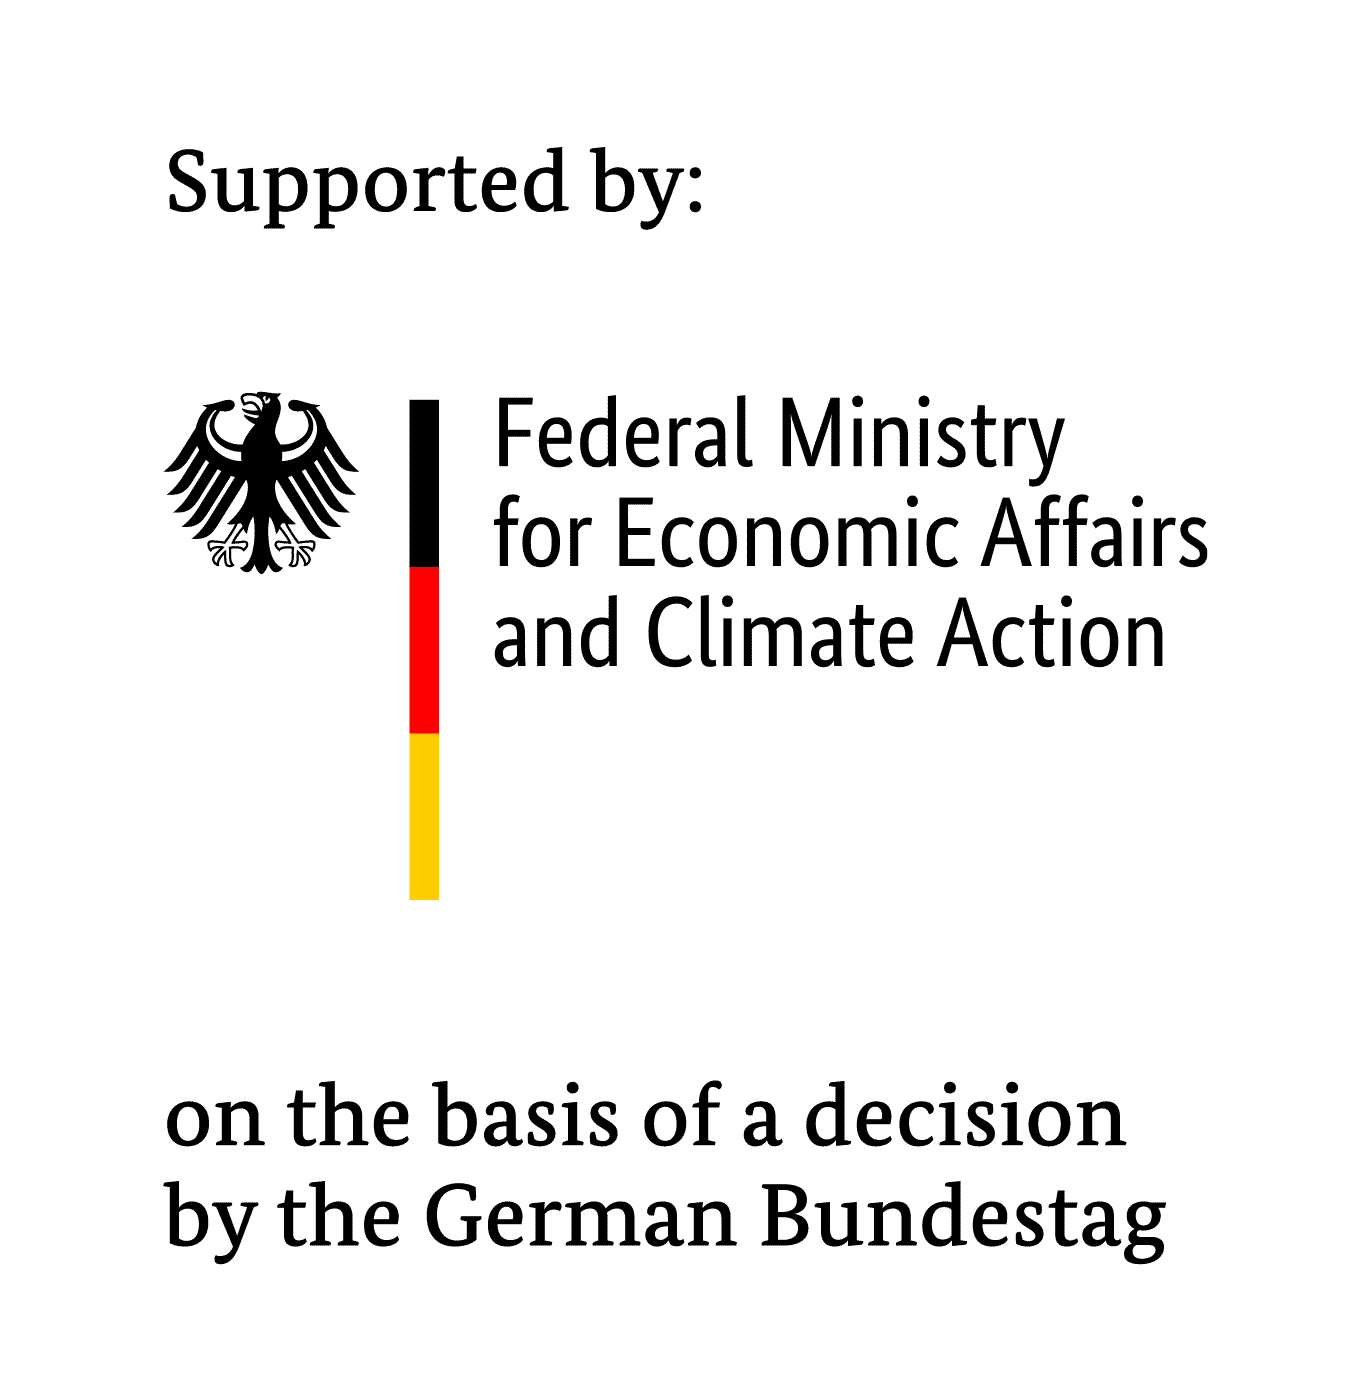
\includegraphics[trim=0.2cm 0.6cm 0.6cm 0.2cm,height=1.1cm,clip=true]{logos/bmwk_en_logo.png}
}


\begin{document}

\addtocounter{framenumber}{-1}
{
  \setbeamertemplate{footline}{
    \usebeamercolor[fg]{framesource}%
    \usebeamerfont{page number in head}%
    \begin{center}
      \Large
      \doclicenseIcon
      \vspace{0.4cm}
    \end{center}
  } 
  \maketitle
}

% \section{Introduction}


% \begin{frame}{RESILIENT project partners}
%   \centering
%   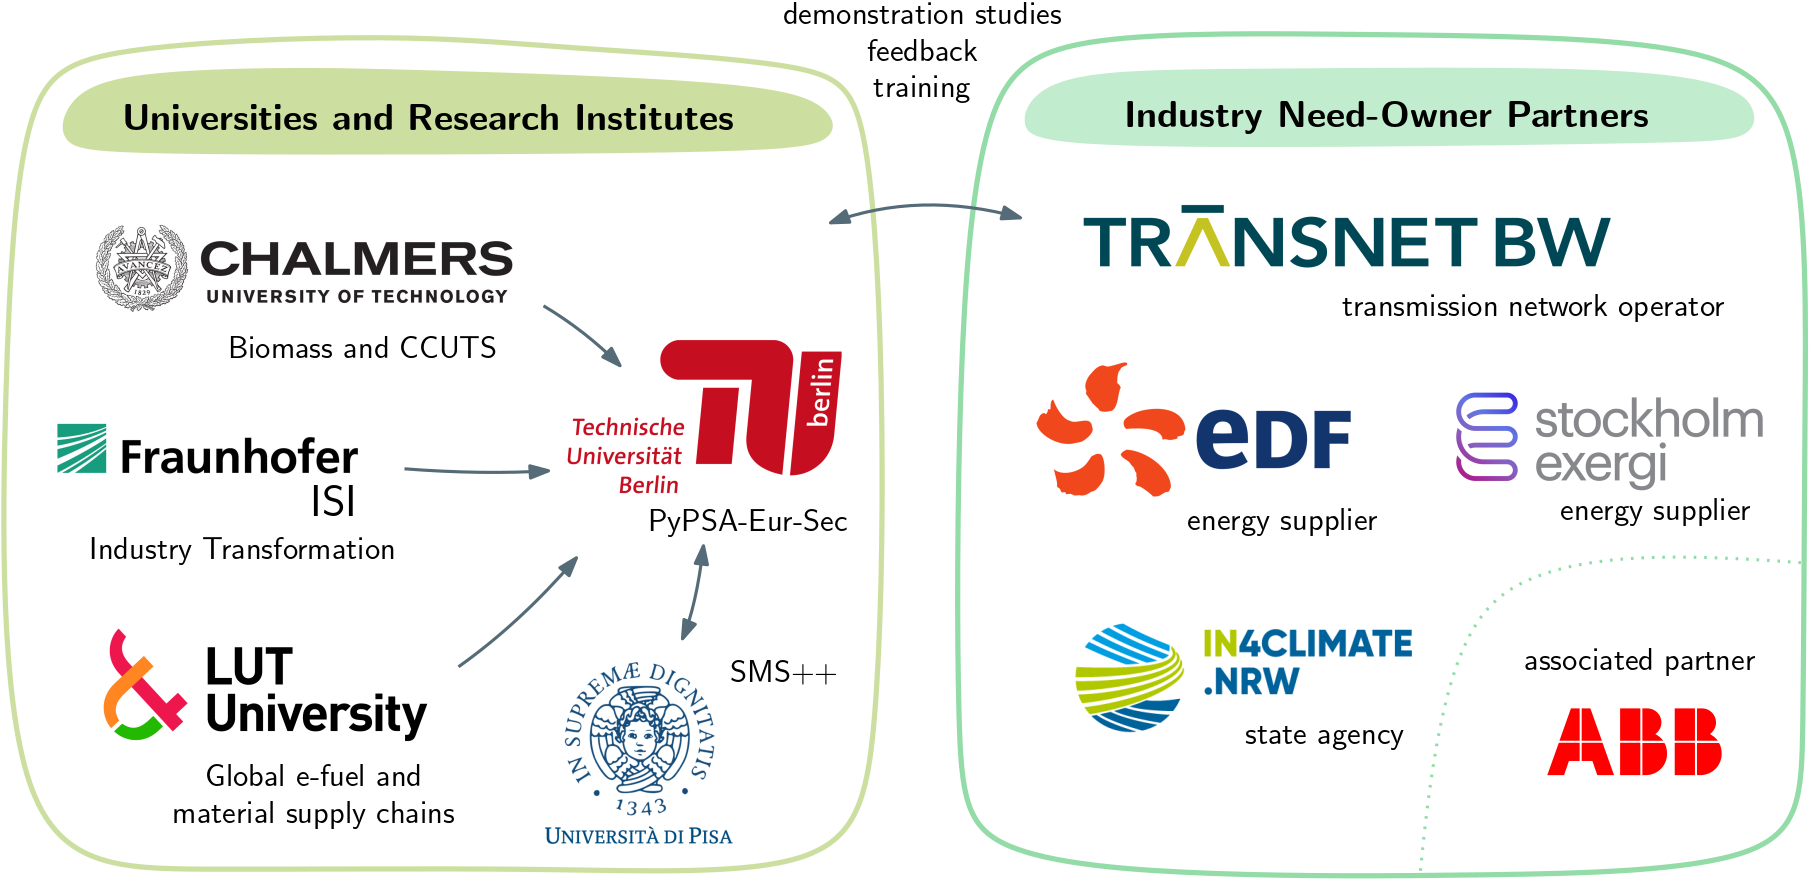
\includegraphics[width=0.85\textwidth]{other/resilient_partners}
  
%   \footnotesize
%   Funded via \alert{CETPartnership 2022} Call --- \alert{BMWK} for all German partners.

%   \source{\url{https://resilient-project.github.io/}}
% \end{frame}

% \begin{frame}{RESILIENT work packages}
%   \centering
%   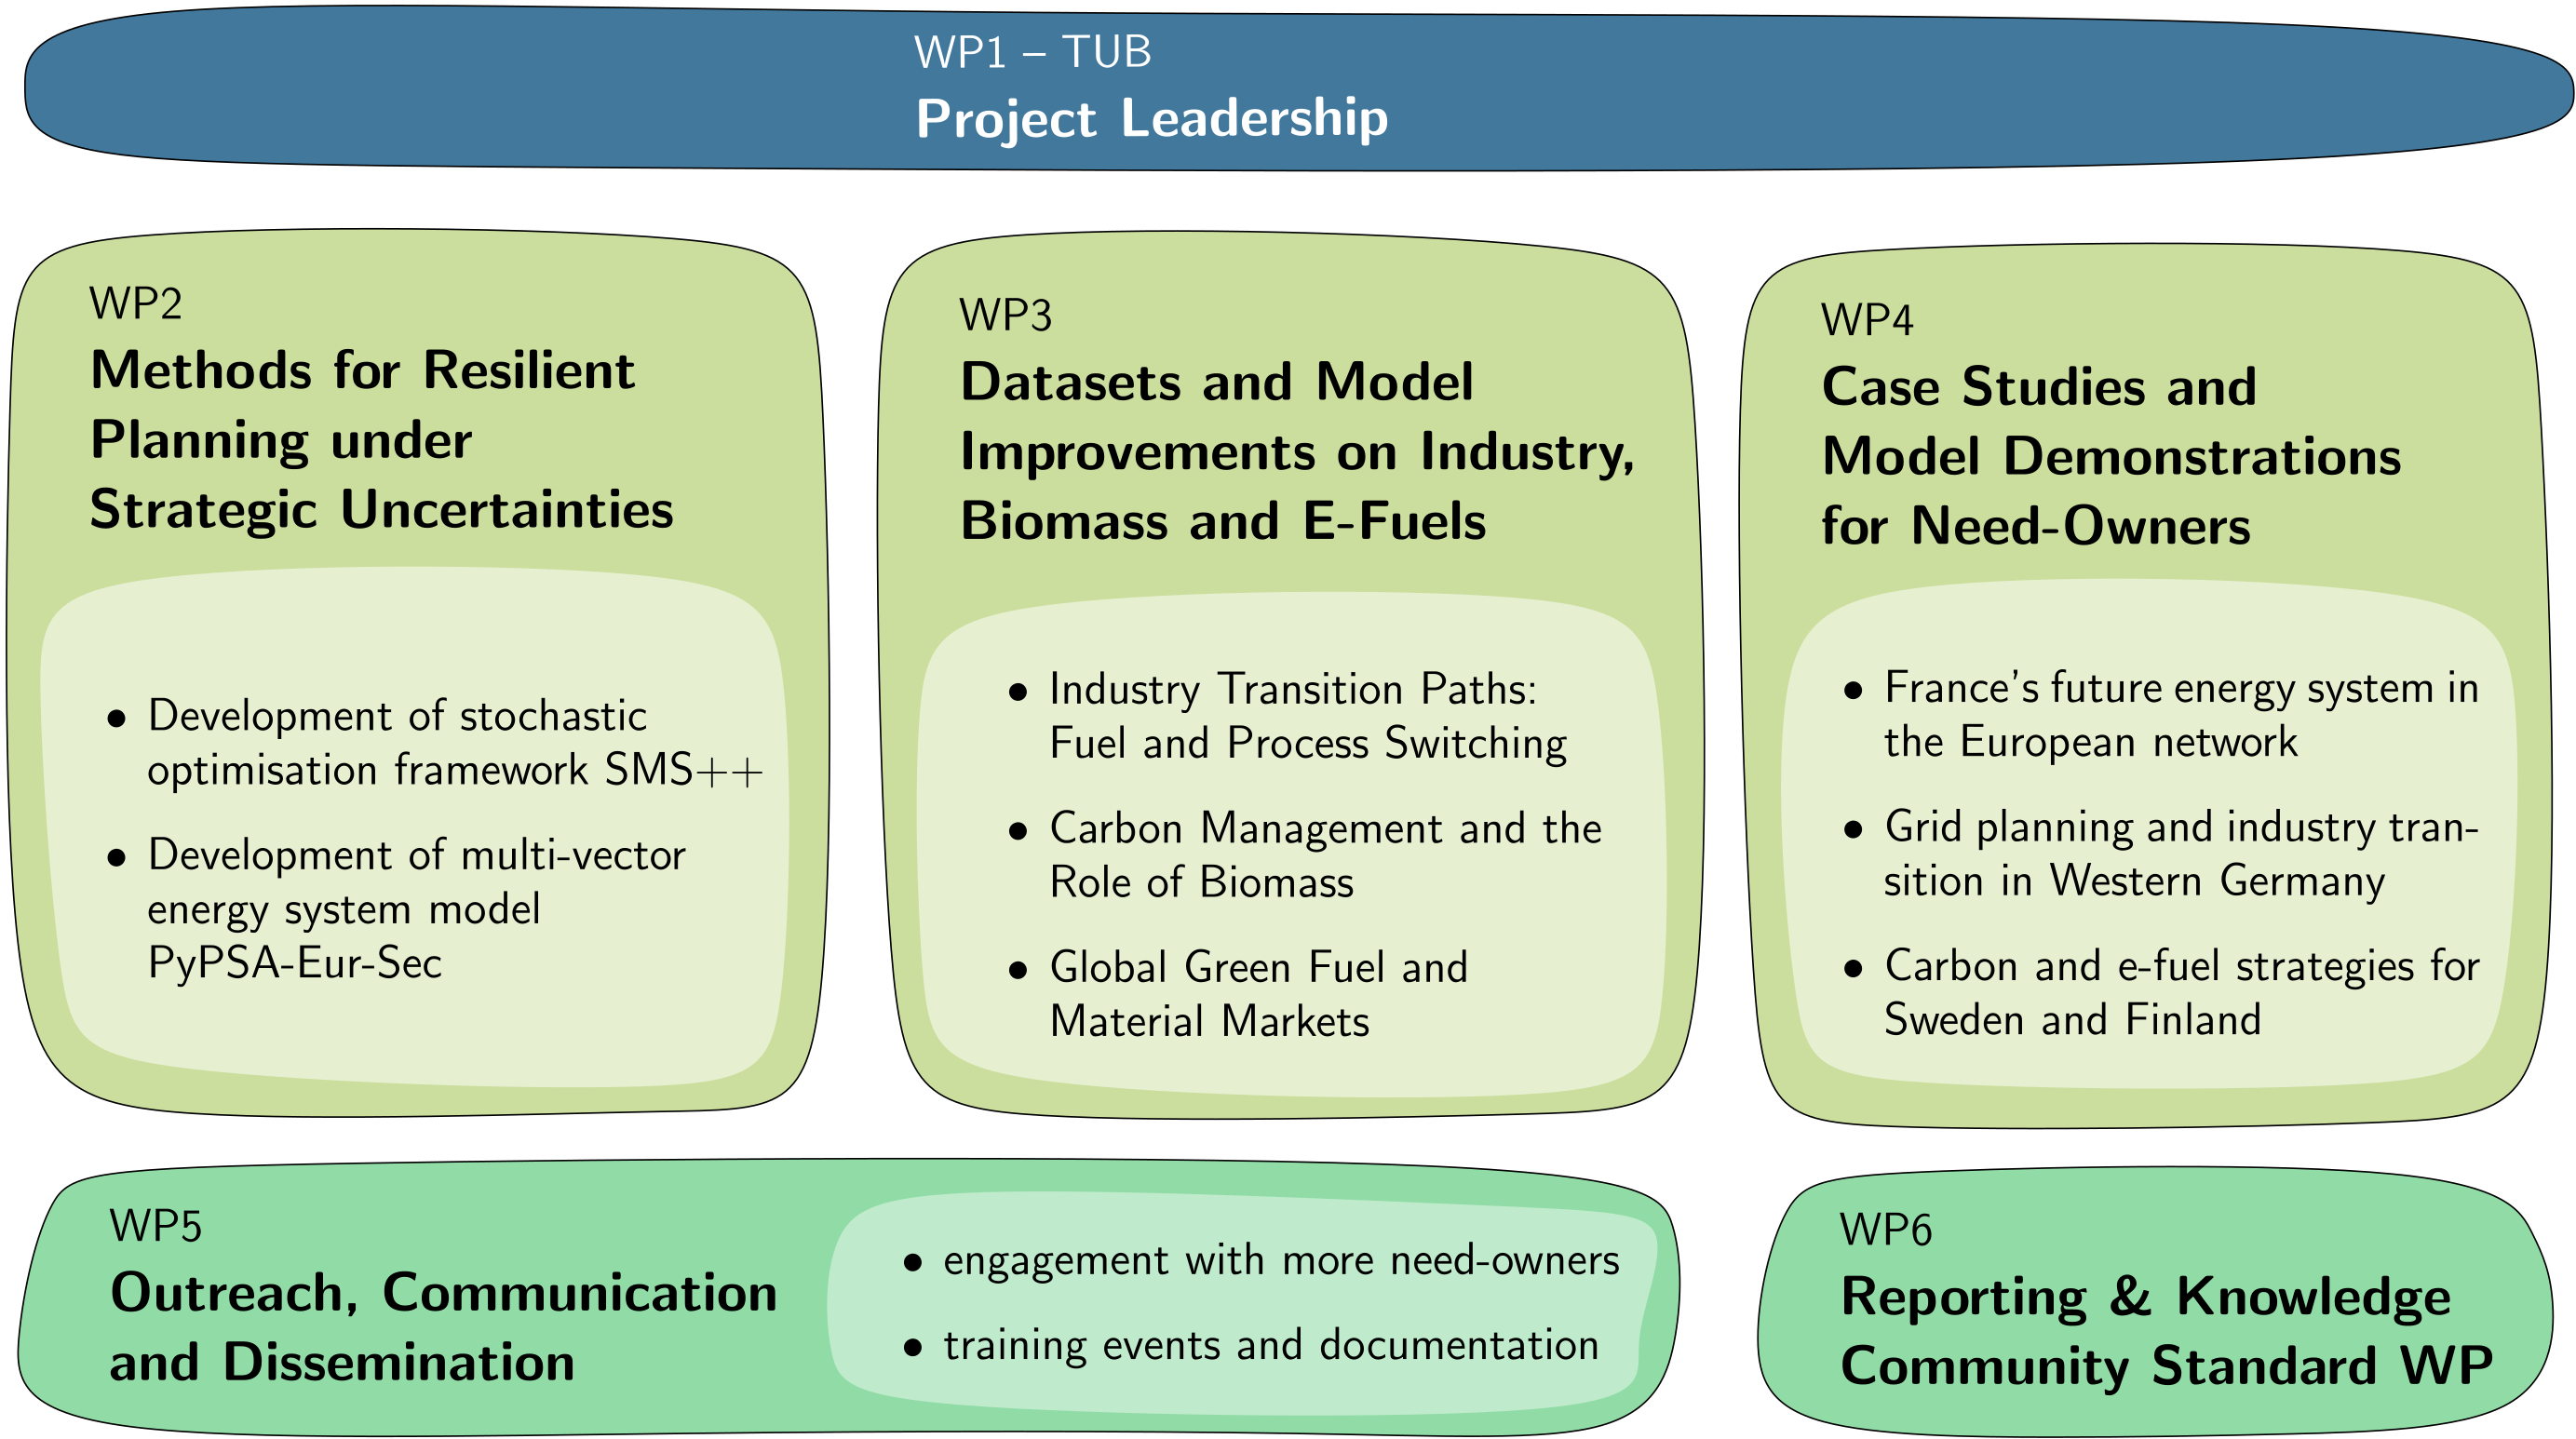
\includegraphics[width=0.8\textwidth]{other/resilient_project_structure}
% \end{frame}

% \begin{frame}{PyPSA-Eur: An open-source, sector-coupled model for Europe}
%   \begin{columns}
%     \begin{column}{0.5\textwidth}
%       \footnotesize
%       \begin{itemize}
%         \setlength\itemsep{.8em}
%         \item Spatially and temporally highly resolved linear optimisation model that covers the \alert{European} continent,
%         \item Built on top of the open-source toolbox \alert{PyPSA},
%         \item Includes \alert{stock} of existing power plants, renewable potentials, availability \alert{time series},
%         \item Covers the \alert{electricity high-voltage grid} from AC 220 kV to 750 kV (UA) and DC 150 kV upwards, option to include planned transmission projects (TYNDP and German NEP),
%         \item Maintained by the Department of Digital Transformation in Energy Systems at \alert{TU Berlin}.
%       \end{itemize}
%     \end{column}
%     \begin{column}{0.5\textwidth}
%       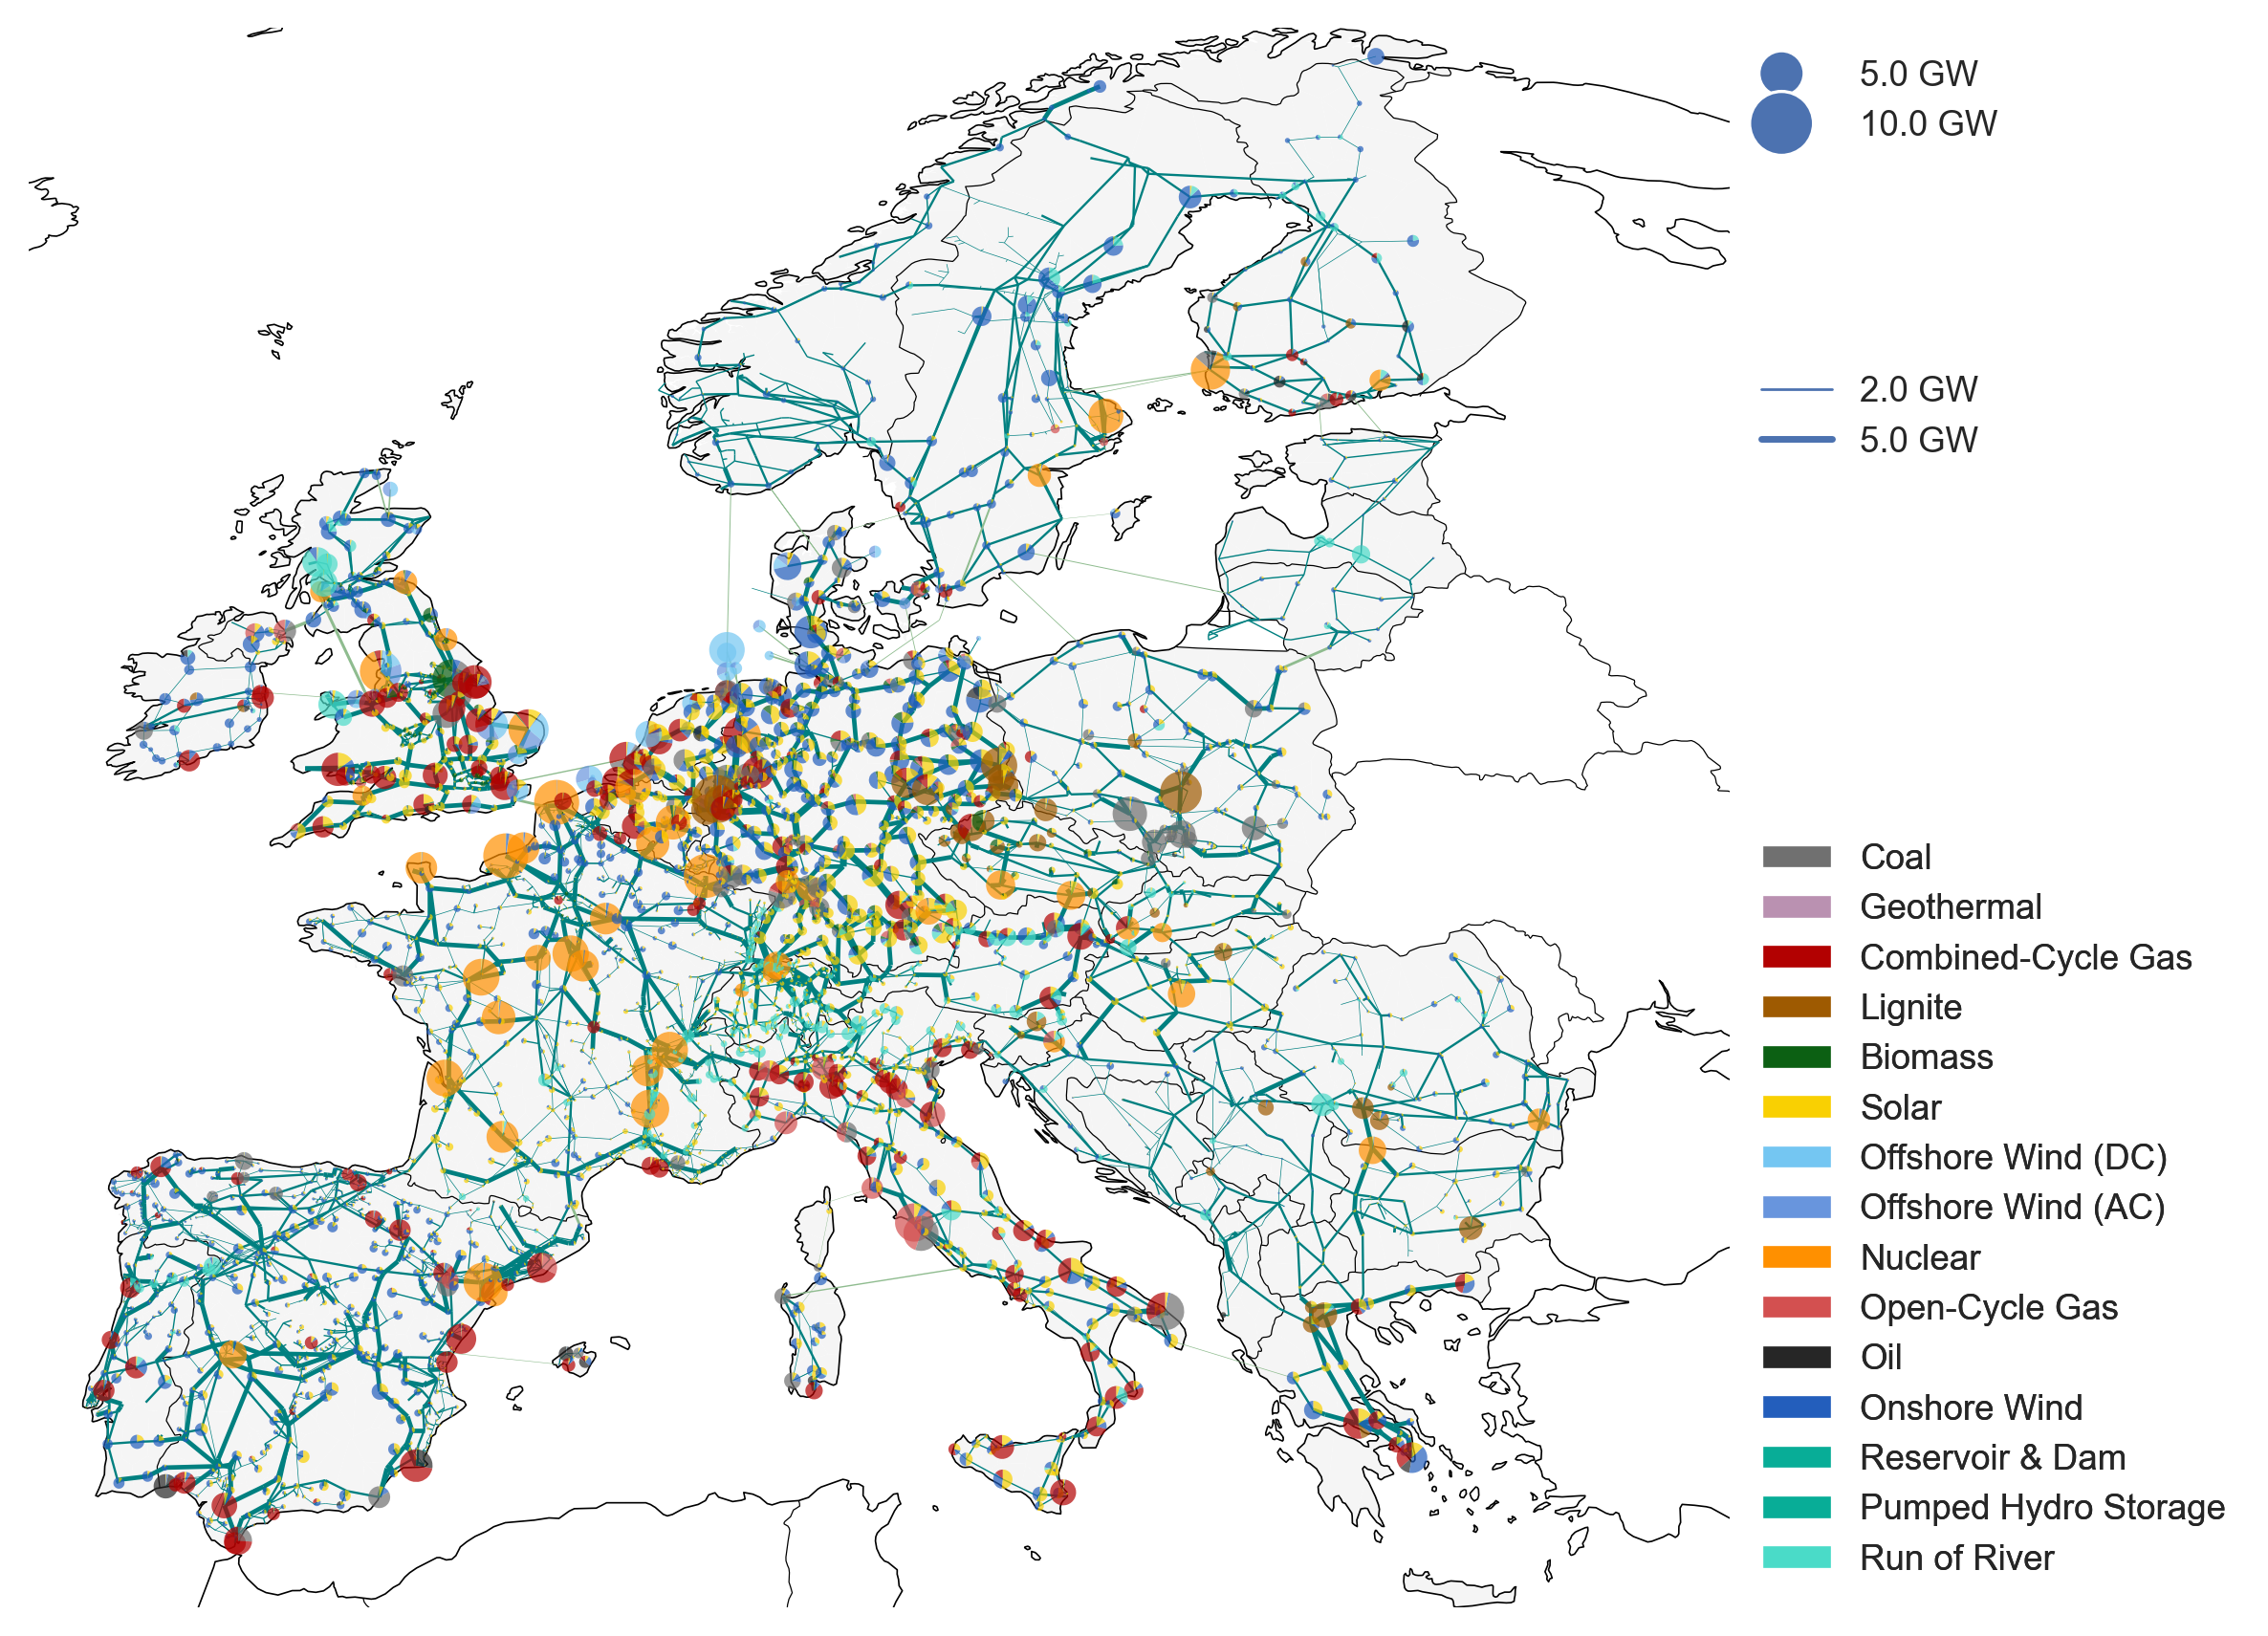
\includegraphics[width=1\textwidth]{other/pypsa_eur_elec}
%     \end{column}
%   \end{columns}

%   \source{\url{https://pypsa-eur.readthedocs.io}}
% \end{frame}

% \begin{frame}{Selection of planned model developments}
%   \footnotesize
%   \begin{columns}[T] % align columns
%     \begin{column}{.5\textwidth}
%         \begin{minipage}[t][.45\textheight]{\linewidth}
%             \begin{alertblock}{\textbf{Computational methods for uncertainties}}
%                 \begin{itemize}
%                   \item decomposition techniques
%                   \item large-scale stochastic optimisation
%                   \item \textbf{test robustness of system}
%                   \item using SMS++ framework
%                 \end{itemize}
%             \end{alertblock}
%         \end{minipage}
        
%         \vspace{-0.03\textheight} % separation between the boxes
        
%         \begin{minipage}[t][.45\textheight]{\linewidth}
%             \begin{alertblock}{\textbf{Industry transformation (FORECAST)}}
%               \begin{itemize}
%                 \item fuel and process switching
%                 \item industry relocation
%                 \item carbon sources and feedstocks
%                 \item data on stock \& investment cycles
%                 \item new technologies (oxyfuel cement, etc.)
%               \end{itemize}
%             \end{alertblock}
%         \end{minipage}
%     \end{column}
    
%     \begin{column}{.5\textwidth}
%         \begin{minipage}[t][.45\textheight]{\linewidth}
%             \begin{alertblock}{\textbf{Carbon management and biomass usage}}
%               \begin{itemize}
%                 \item \textbf{CO$_2$ network}
%                 \item \textbf{CO$_2$ sequestration potentials}
%                 \item circular carbon economy and recycling
%                 \item biomass usage options
%               \end{itemize}
%             \end{alertblock}
%         \end{minipage}
        
%         \vspace{-0.03\textheight} % separation between the boxes
        
%         \begin{minipage}[t][.45\textheight]{\linewidth}
%             \begin{alertblock}{\textbf{Global green fuel and material markets}}
%               \begin{itemize}
%                 \item \textbf{imports of green energy and materials}
%                 \item \textbf{effects on European infrastructure}
%                 \item restructuring of value chains
%                 \item risks (geopolitical, technological, etc.) \newline
%               \end{itemize}
%             \end{alertblock}
%         \end{minipage}
%     \end{column}
% \end{columns}
% \end{frame}

\section{Introduction \& Background}
\begin{frame}{Motivation: 2030 policy targets}
  \footnotesize

  The EU has set ambitious targets for 2030, including the electricity, hydrogen and CO$_2$ infrastructure sector.

  \begin{columns}[T] % align columns
    % First column
    \begin{column}{.3\textwidth}
        \begin{minipage}[t][.45\textheight]{\linewidth}
            \begin{alertblock}{\textbf{55 \% emission reduction}}
                \begin{itemize}
                  \item \alert{Fit for 55}
                  \item Translating to an emission allowance of ca. 2 bn. t CO$_2$ p.a. in 2030
                  \item Covering the electricity, heat, industry, transport, buildings and agriculture sectors \newline
                \end{itemize}
                \vspace{0.06cm}
            \end{alertblock}
        \end{minipage}
    \end{column}
    
    % Second column
    \begin{column}{.34\textwidth}
        \begin{minipage}[t][.45\textheight]{\linewidth}
            \begin{exampleblock}{\textbf{10 Mt p.a. green H$_2$ production}}
                \begin{itemize}
                  \item \alert{REPowerEU}
                  \item Accelerating the transition away from fossil fuels (esp. Russian gas), enhancing energy security through renewables
                  \item Aligns with European Green Deal and targets scaling up renewable H$_2$ in hard-to-electrify-sectors
                \end{itemize}
            \end{exampleblock}
        \end{minipage}
    \end{column}

    % Third column
    \begin{column}{.3\textwidth}
        \begin{minipage}[t][.45\textheight]{\linewidth}
            \begin{exampleblock}{\textbf{50 Mt p.a. CO$_2$ sequestration}}
                \begin{itemize}
                  \item \alert{Net-Zero Industry Act}
                  \item Essential component in helping industries to reduce their net emissions
                  \item Provides means to capture unavoidable emissions from hard-to-abate sectors like cement, steel, chemicals, etc.
                \end{itemize}
            \end{exampleblock}
        \end{minipage}
    \end{column}
  \end{columns}

  \vspace{1.3cm}

\end{frame}

\begin{frame}{Motivation: PCI-PMI projects}
  \scriptsize
  \begin{columns}[T] % align columns
    % First column
    \begin{column}{.63\textwidth}
        \begin{minipage}[t][.45\textheight]{\linewidth}
            \begin{alertblock}{\textbf{What are PCI-PMI projects?}}
                \begin{itemize}
                  \setlength\itemsep{0.85em}
                  \item Projects of Common Interest (PCIs) are key \alert{cross-border infrastructure projects} that link the energy systems of EU countries
                  \item Projects of Mutual Interest (PMIs) include cooperations with countries outside the EU
                  \item Intend ``to help the EU achieve its \alert{energy policy and climate objectives}: affordable, secure and sustainable energy for all citizens and the long-term decarbonisation of the economy in accordance with the \alert{Paris Agreement}''
                  \item ``Potential overall benefits of the project must outweigh its costs'' 
                  \item Given their \alert{lighthouse character}, these projects are highly likely to be implemented. 
                  \item Large infrastructure projects (incl. PCI-PMI) are however commonly facing delays due to permitting, procurement bottlenecks, etc.
                \end{itemize}
            \end{alertblock}
        \end{minipage}
    \end{column}
    
    % Second column
    \begin{column}{.36\textwidth}
        \begin{minipage}[t][.45\textheight]{\linewidth}
            \begin{alertblock}{\textbf{Project map}}
              \centering
              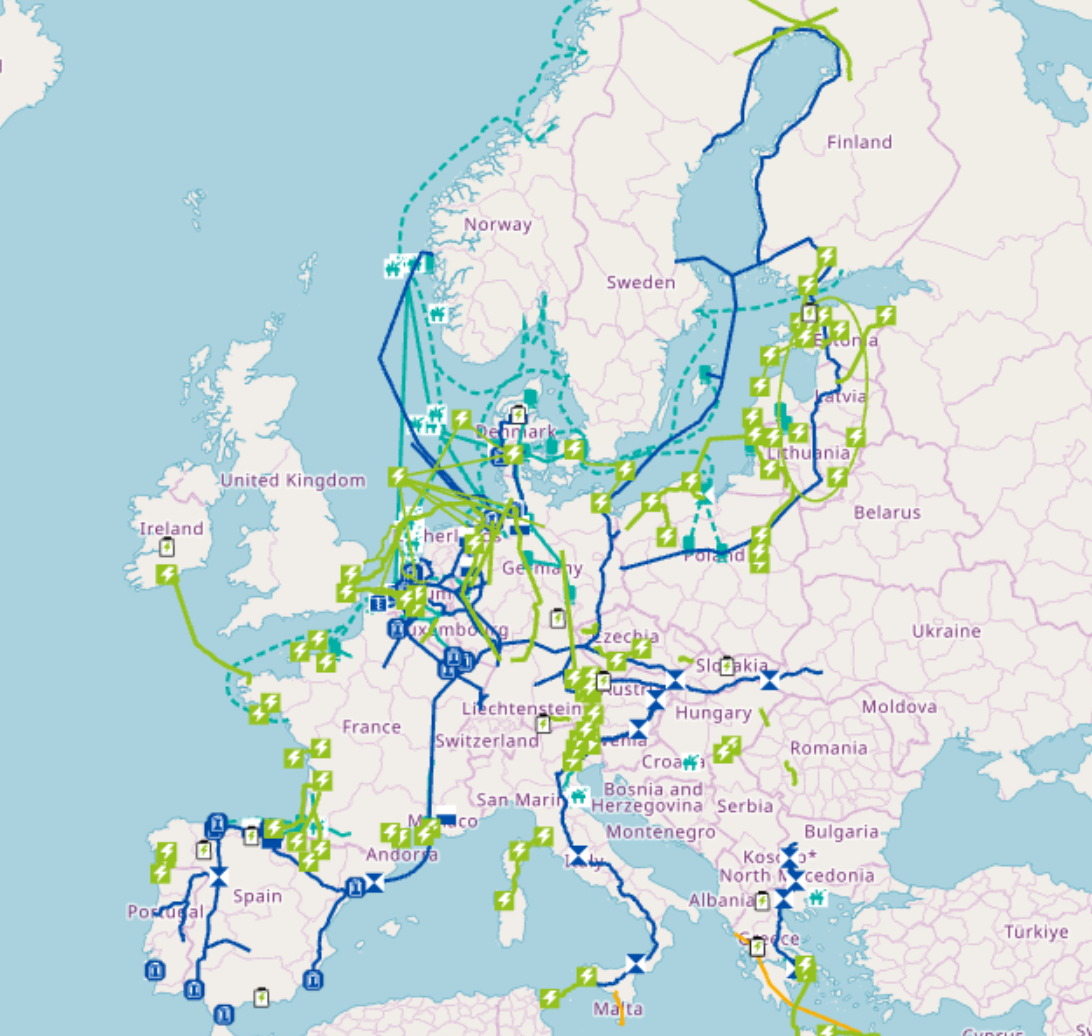
\includegraphics[width=1\textwidth]{pci_pmi_map}
            \end{alertblock}
        \end{minipage}
    \end{column}

  \end{columns}

  \vspace{2.1cm}

\begin{enumerate} 
  \item What is the long-term value of PCI-PMI projects in supporting the EU’s climate and energy policy targets, and what are the associated costs?
  \item What are the costs of adhering to the EU policy targets, even when the implementation of PCI-PMI projects is delayed?
\end{enumerate}

  \source{\url{https://energy.ec.europa.eu/topics/infrastructure_en} \\ and \url{https://ec.europa.eu/energy/infrastructure/transparency_platform/map-viewer}}

\end{frame}


\section{Methodology}

\begin{frame}{Model setup}
  \begin{columns}
    \begin{column}{0.55\textwidth}
      \footnotesize
      \begin{itemize}
        \setlength\itemsep{.8em}
        \item Including sectors \alert{power, heat, transport, industry, feedstock} and \alert{agriculture}
        \item \alert{Myopic optimisation} for 2030, 2040 and 2050
        \item \alert{Co-optimising} generation, transmission, storage, and power-to-X conversion
        \item Resolving 34 countries to \alert{99 regions} (NUTS mix) at \alert{4-hourly} temporal resolution on avg. (using tsam).
        \item Implementing \alert{PCI-PMI} HVAC, HVDC, hydrogen and carbon infrastructure projects as well as key GHG, \ce{H2} production, electrolyser capacity, and \ce{CO2} sequestration targets (next slide). Additional sequestration potential from \alert{depleted oil and gas fields} \cite{hofmannH2CO2Network2025}
        \item \alert{Regret analysis} approach based on 5 long-term scenario, 3 short-term scenarios, in total 60 model runs
      \end{itemize}
    \end{column}
    \begin{column}{0.45\textwidth}
      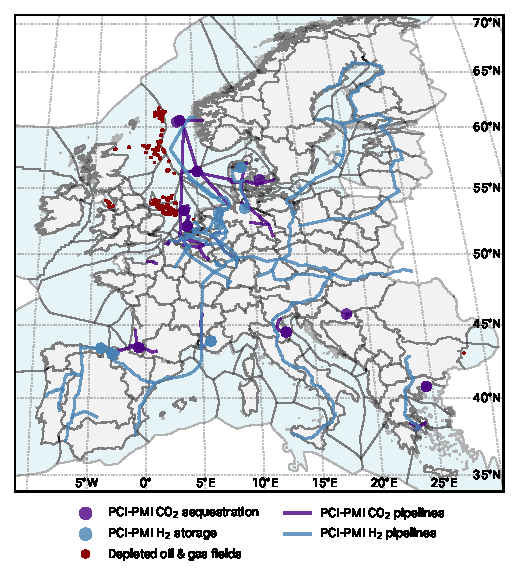
\includegraphics[width=1\textwidth]{map_adm_pcipmi}
    \end{column}
  \end{columns}
  \source{Own illustration based on data extracted from \url{https://ec.europa.eu/energy/infrastructure/transparency_platform/map-viewer}}
\end{frame}

\begin{frame}{Exogenous demand}
  \centering
  \begin{columns}
    \begin{column}{0.48\textwidth}
      \footnotesize
      \begin{figure}
        \centering
        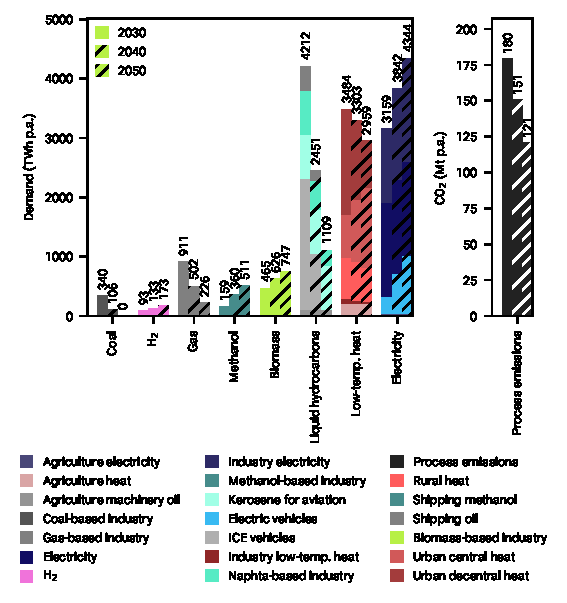
\includegraphics[width=1\textwidth]{exogenous_demand}
      \end{figure}
    \end{column}
    \begin{column}{0.52\textwidth}
      \footnotesize
      \begin{itemize}
        \item Demand for electricity, heat, gas, biomass, and transport is regionally and temporally resolved
        \item ICE vehicles in land transport expected to fully phase out in favour of EV by 2050
        \item Demand for methanol and hydrocarbons, including kerosene primarily driven by shipping, aviation, and industry sector (not spatially resolved)
        \item Unabatable process emissions from industry sector, e.g. cement, also considered
        \item \ce{CO2} sequestration cost assumed at \euro{15}/t\ce{CO2} (mid-range estimate)
      \end{itemize}
    \end{column}
  \end{columns}
  \source{Own illustration.}
\end{frame}


\begin{frame}{Long-term scenarios: Implemented targets}
  \scriptsize
  \begin{tabularx}{0.8\textwidth}{R{3.9cm}>{\centering\arraybackslash}X>{\centering\arraybackslash}X>{\centering\arraybackslash}X}
    \toprule
    \textbf{Planning horizon} & \textbf{2030} & \textbf{2040} & \textbf{2050} \\
    \midrule
    \textbf{Targets} & & & \\
    GHG emission reduction &  \SI{-55}{\percent} & \SI{-90}{\percent} & \SI{-100}{\percent} \\
    \ce{CO2} sequestration & 50 Mt p.a. & 150 Mt p.a. & 250 Mt p.a. \\
    Electrolytic \ce{H2} production & 10 Mt p.a. & 27.5 Mt p.a. & 45 Mt p.a. \\
    \ce{H2} electrolyser capacity & \SI{40}{GW} &  \SI{110}{GW} &  \SI{180}{GW} \\
    \bottomrule
  \end{tabularx}
  \scriptsize 
  \centering
  \newline
  Model targets based on \cite{europeancommissionFit55Delivering2021,europeancommissionREPowerEUPlanCommunication2022,europeanparliamentRegulationEU20242024,europeancommissionCommunicationCommissionEuropean2024,europeancommission.directorategeneralforenergy.METIS3Study2023}
  \source{Own illustration.}
\end{frame}



\begin{frame}{Long-term scenarios: Definition}
  \scriptsize
  \begin{tabularx}{0.8\textwidth}{R{3.9cm}>{\centering\arraybackslash}X>{\centering\arraybackslash}X>{\centering\arraybackslash}X>{\centering\arraybackslash}X>{\centering\arraybackslash}X}
      \toprule
      \textbf{Long-term scenarios} & 
      \textbf{DI} & 
      \textbf{PCI} & 
      \textbf{PCI-n} & 
      \textbf{PCI-in} & 
      \textbf{CP} \\
      \midrule
      \textbf{\ce{CO2} sequestration} & & & & & \\
      Depleted oil \& gas fields* & $\blacksquare$ & $\blacksquare$ & $\blacksquare$ & $\blacksquare$ & $\blacksquare$ \\
      PCI-PMI seq. sites** & -- & $\blacksquare$ & $\blacksquare$ & $\blacksquare$ & $\blacksquare$ \\
      \midrule
      \textbf{\ce{H2} storage} & & & & & \\
      Endogenous build-out & $\blacksquare$ & $\blacksquare$ & $\blacksquare$ & $\blacksquare$ & $\blacksquare$ \\
      PCI-PMI storage sites & -- & $\blacksquare$ & $\blacksquare$ & $\blacksquare$ & $\blacksquare$ \\
      \midrule
      \textbf{\ce{CO2} pipelines} & & & & & \\
      to depleted oil \& gas fields & $\blacksquare$ & $\blacksquare$ & $\blacksquare$ & $\blacksquare$ & $\blacksquare$ \\
      to PCI-PMI seq. sites & -- & $\blacksquare$ & $\blacksquare$ & $\blacksquare$ & $\blacksquare$ \\
      \midrule
      \textbf{\ce{CO2} and \ce{H2} pipelines} & & & & & \\
      PCI-PMI & -- & $\blacksquare$ & $\blacksquare$ & $\blacksquare$ & $\blacksquare$ \\
      National build-out & -- & $\blacksquare$ & $\blacksquare$ & $\blacksquare$ & $\blacksquare$ \\
      International build-out & -- & -- & -- & $\blacksquare$ & $\blacksquare$ \\
      PCI-PMI extendable & -- & -- & -- & -- & $\blacksquare$ \\
      \bottomrule
  \end{tabularx}
  \source{Own illustration.}
  \vspace{0.5em}
  \centering
  \newline
  {\scriptsize $\blacksquare$ enabled \quad -- disabled \quad * approx. 286 Mt p.a. \quad ** approx. 114 Mt p.a.}
\end{frame}

\begin{frame}{Regret matrix setup}
  \scriptsize
  \begin{tabularx}{0.8\textwidth}{R{3.9cm}>{\centering\arraybackslash}X>{\centering\arraybackslash}X>{\centering\arraybackslash}X}
    \toprule
    \textbf{Short-term} & \textbf{Reduced targets} & \textbf{Delayed pipelines} & \textbf{No pipelines} \\
    \midrule
    \textbf{Long-term scenarios} & & & \\
    Decentral Islands (\textbf{DI}) & $\blacksquare$ & -- & -- \\
    PCI-PMI (\textbf{PCI}) & $\blacksquare$ & $\blacksquare$ & $\blacksquare$ \\
    PCI-PMI nat. (\textbf{PCI-n}) & $\blacksquare$ & $\blacksquare$ & $\blacksquare$\\
    PCI-PMI internat. (\textbf{PCI-in}) & $\blacksquare$ & $\blacksquare$ & $\blacksquare$ \\
    Central Planning (\textbf{CP}) & $\blacksquare$ & $\blacksquare$ & $\blacksquare$ \\
    \midrule
    \textbf{Targets} & & & \\
    GHG emission reduction &  $\blacksquare$ &  $\blacksquare$ &  $\blacksquare$ \\
    \ce{CO2} sequestration &  -- &  $\blacksquare$ &  $\blacksquare$ \\
    Electrolytic \ce{H2} production &  -- &  $\blacksquare$ &  $\blacksquare$ \\
    \ce{H2} electrolysers &  -- &  $\blacksquare$ &  $\blacksquare$ \\
    \midrule
    \textbf{\ce{CO2} + \ce{H2} infrastructure} & & & \\
    \ce{CO2} sequestration sites & $\blacksquare$ &  $\blacksquare$ &  $\blacksquare$ \\
    \ce{CO2} pipelines to seq. site & $\blacksquare$ &  $\blacksquare$ &  $\blacksquare$ \\
    \ce{CO2} pipelines & $\blacksquare$ &  $\square$ &  -- \\
    \ce{H2} pipelines & $\blacksquare$ &  $\square$ &  -- \\
    \bottomrule
  \end{tabularx}
  \source{Own illustration.}
  \centering
  \newline
  \scriptsize $\blacksquare$ enabled \quad $\square$ delayed by one period \quad -- disabled

\end{frame}
\section{Results \& Discussion}

\begin{frame}{LT --- Total system costs}
  \centering
  \begin{columns}
    \begin{column}{0.48\textwidth}
      \footnotesize
      \begin{figure}
        \centering
        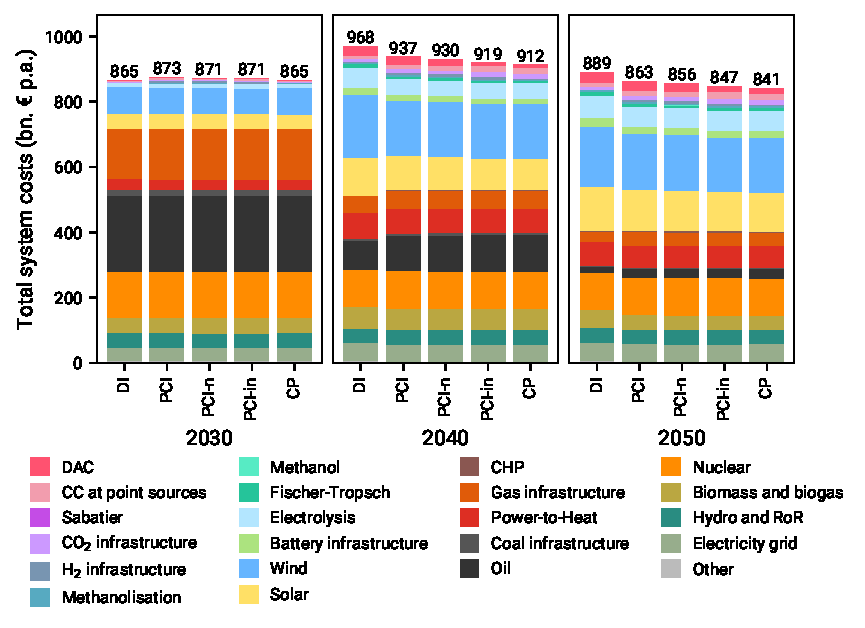
\includegraphics[width=1\textwidth]{costs_overview}
      \end{figure}
    \end{column}
    \begin{column}{0.52\textwidth}
      \footnotesize
      \begin{itemize}
        \item Highest total annual system costs in 2040: \euro{912}-\euro{968} billion per year, driven by sharp decarbonisation pathway
        \item Adding PCI-PMI projects in 2030 increases costs only marginally
        \item Strong system cost savings from pipeline investments starting in 2040, around \euro{30}-\euro{50} billion per year
        \item Complete freedom in pipeline expansion unlocks another \euro{7} billion per year in cost savings
        \item Cost savings stem primarily from reducing reliance into costly DAC technologies and excessive investments into solar and wind
      \end{itemize}
    \end{column}
  \end{columns}
  \source{Own illustration.}
\end{frame}

\begin{frame}{LT --- PCI: 2030 regional \ce{H2}, \ce{CO2} balances, transport, and prices}
  \centering
  \begin{columns}
    \begin{column}{0.5\textwidth}
      \footnotesize
      \begin{figure}
        \centering
        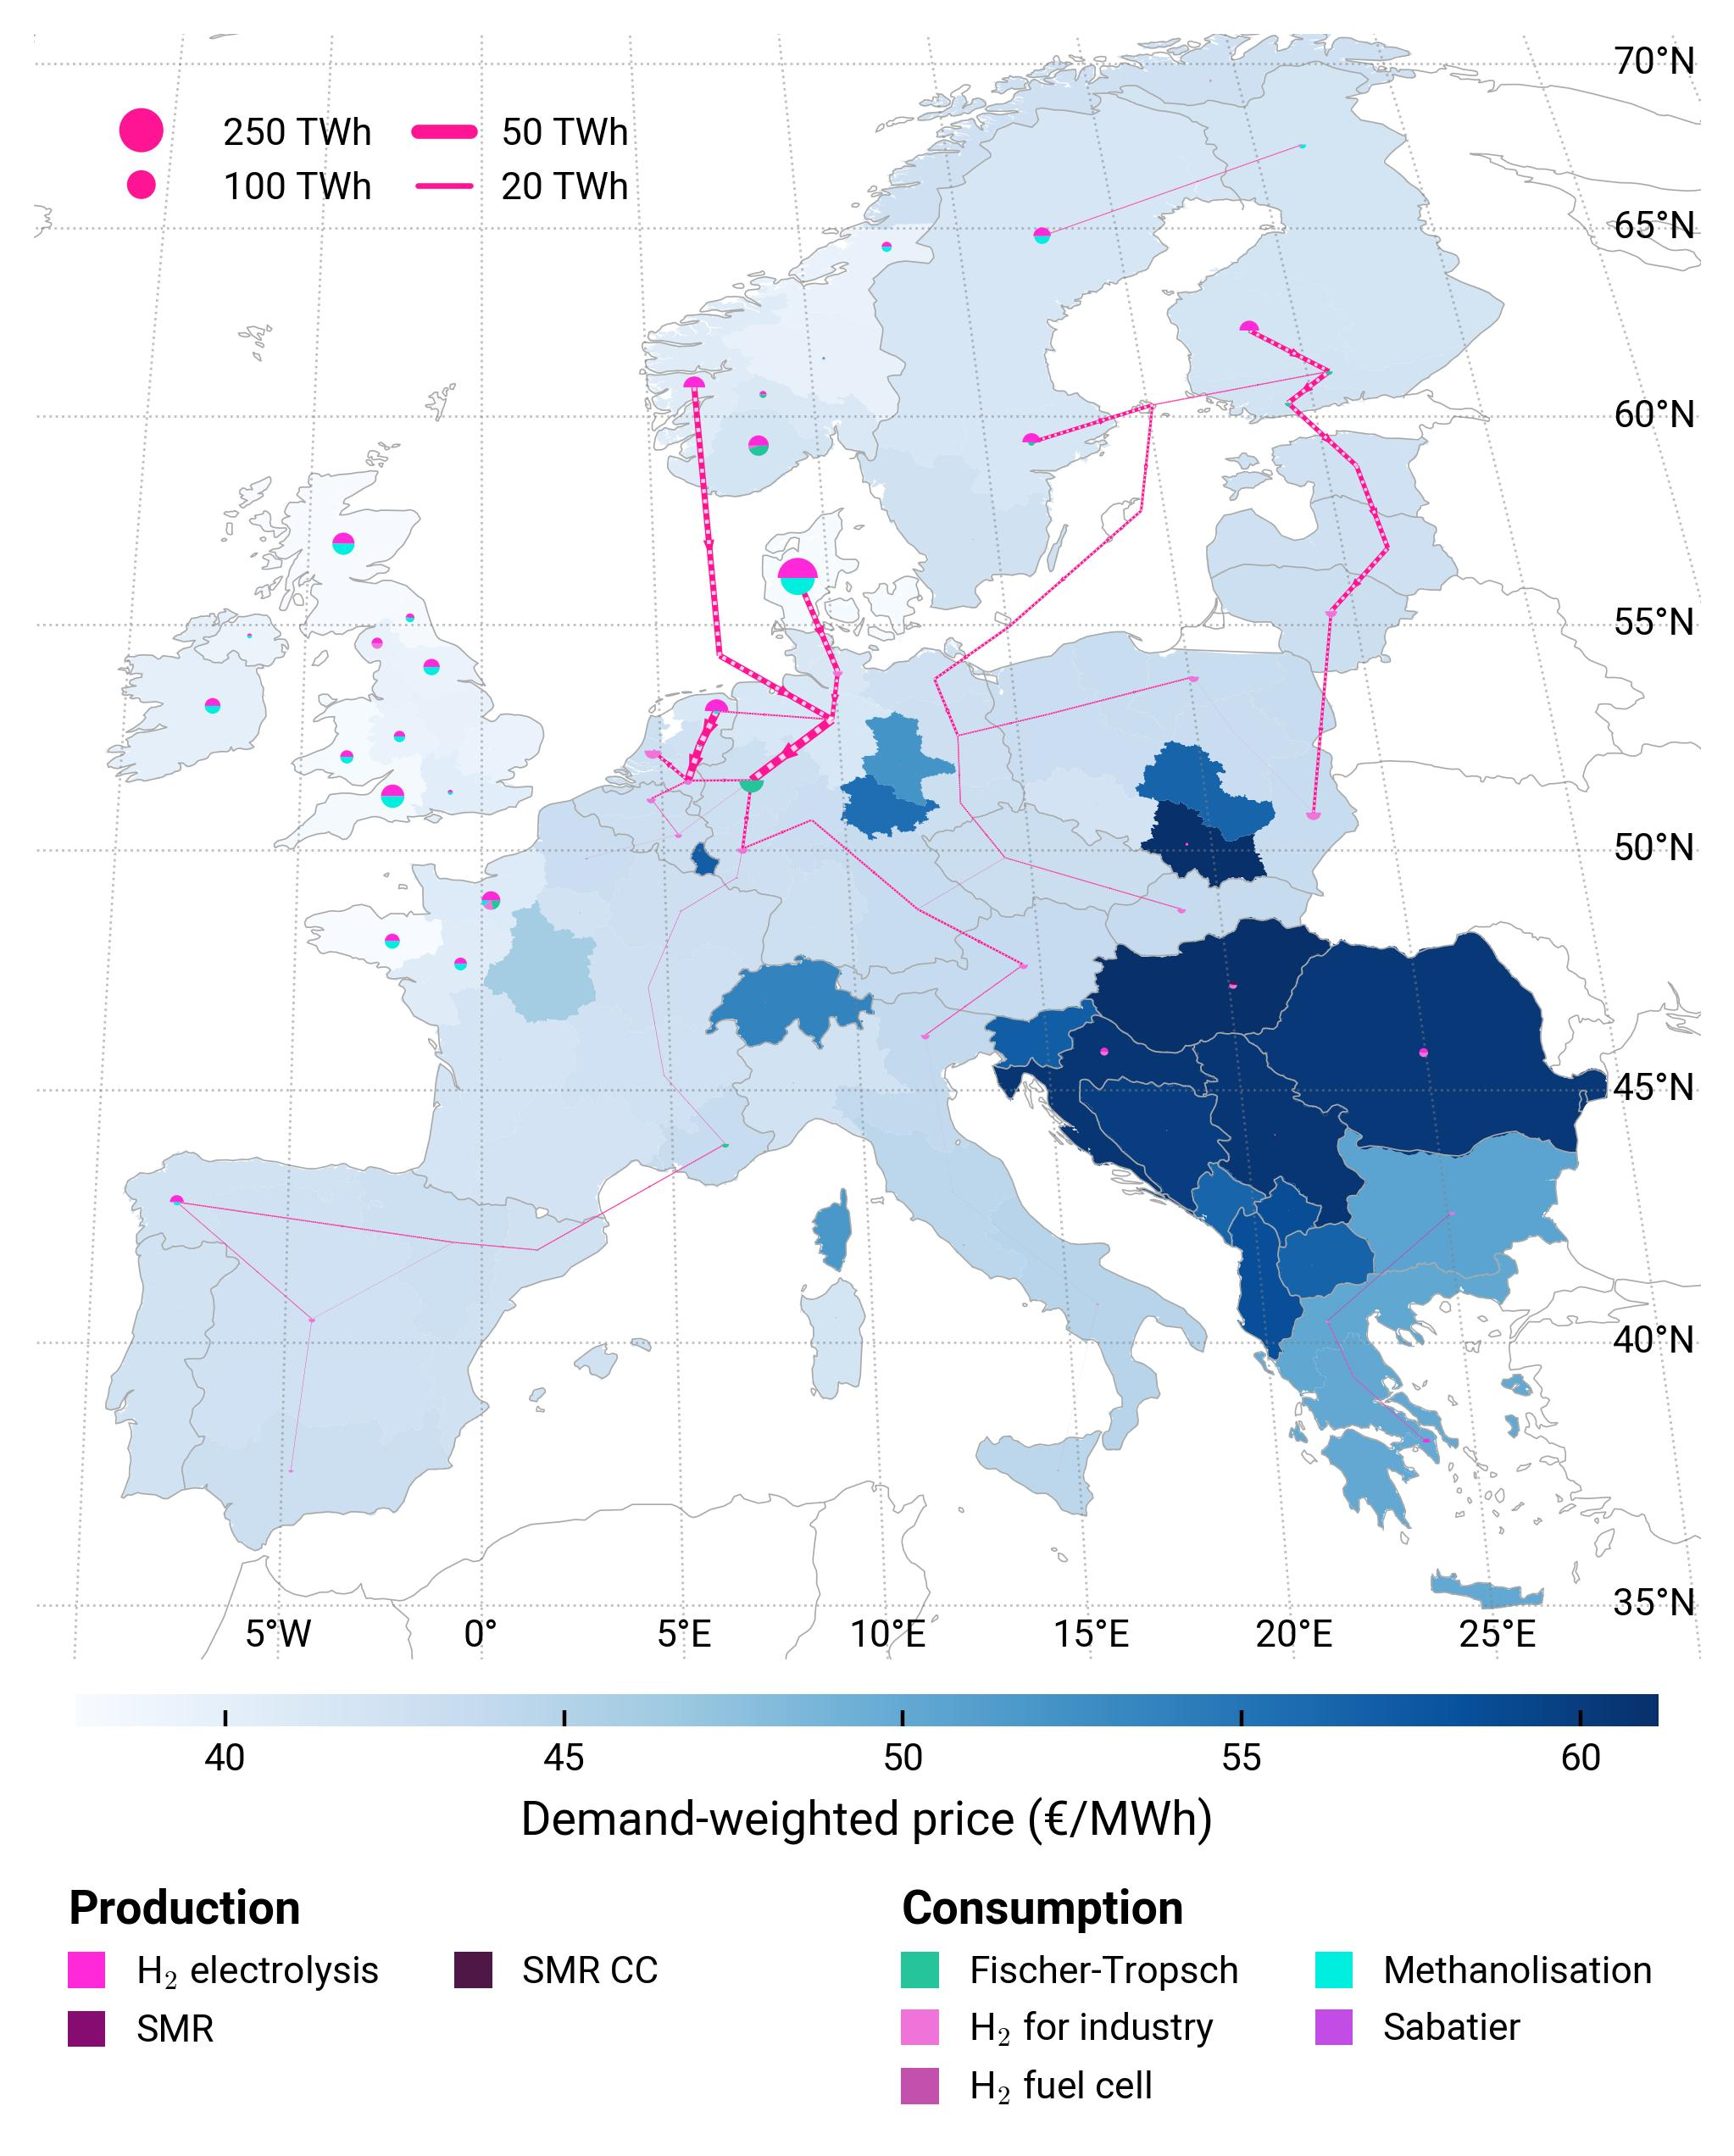
\includegraphics[width=0.76\textwidth]{maps/pcipmi/base_s_adm___2030-balance_map_H2}
      \end{figure}
    \end{column}
    \begin{column}{0.5\textwidth}
      \begin{figure}
        \centering
        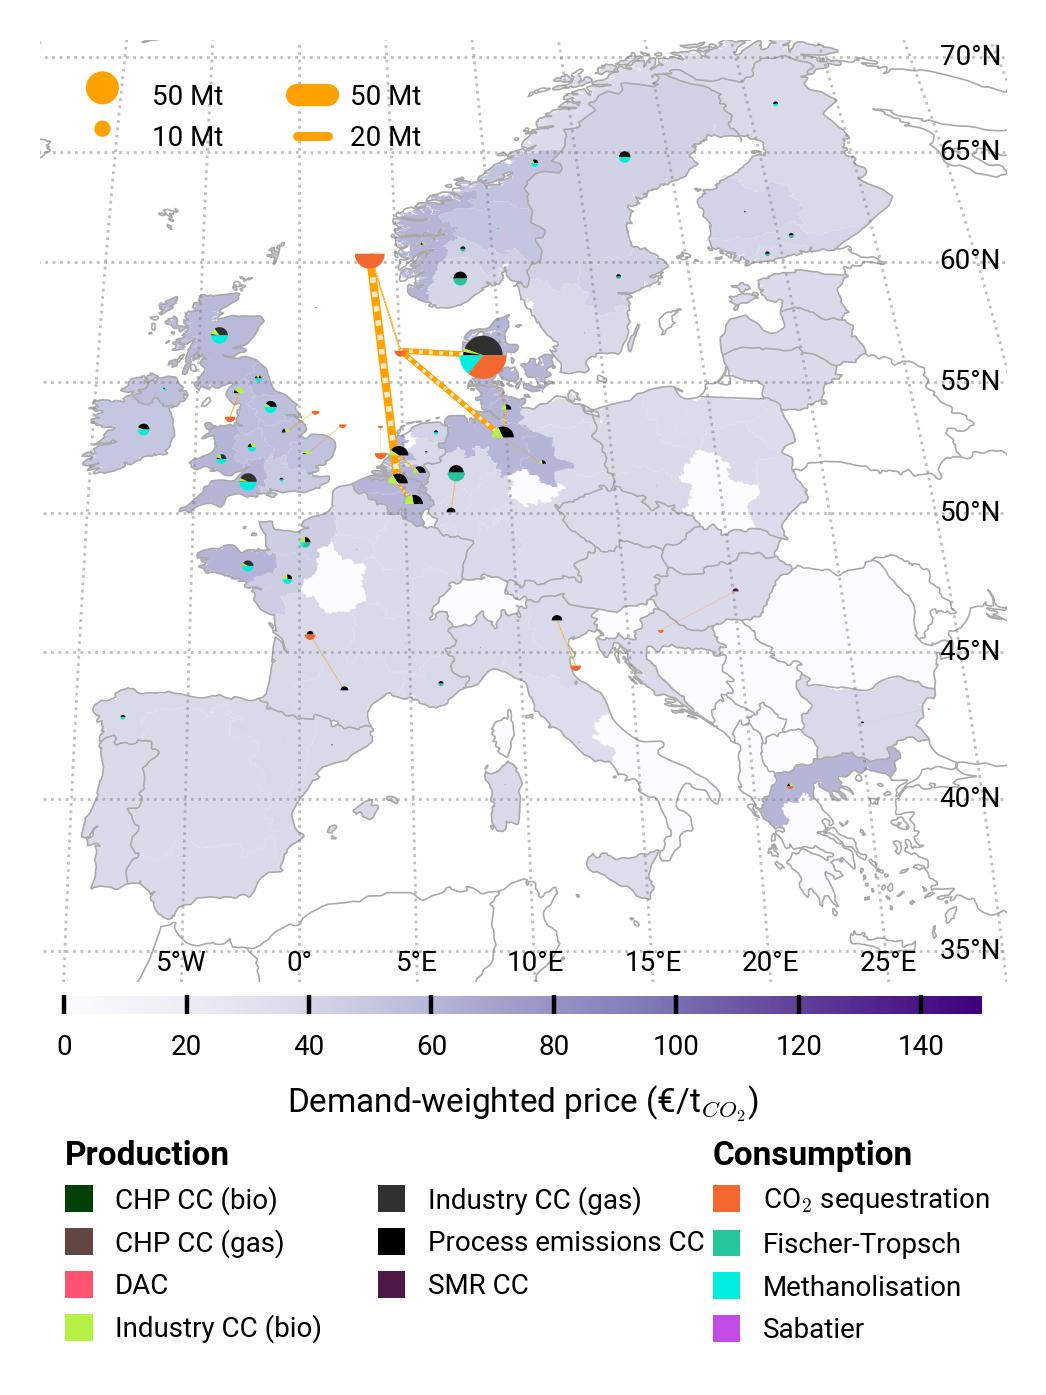
\includegraphics[width=0.76\textwidth]{maps/pcipmi/base_s_adm___2030-balance_map_co2_stored}
      \end{figure}
    \end{column}
  \end{columns}
  \source{Own illustration.}
\end{frame}

% \begin{frame}{LT --- PCI: 2040 regional \ce{H2}, \ce{CO2} balances and transport}
%   \centering
%   \begin{columns}
%     \begin{column}{0.5\textwidth}
%       \footnotesize
%       \begin{figure}
%         \centering
%         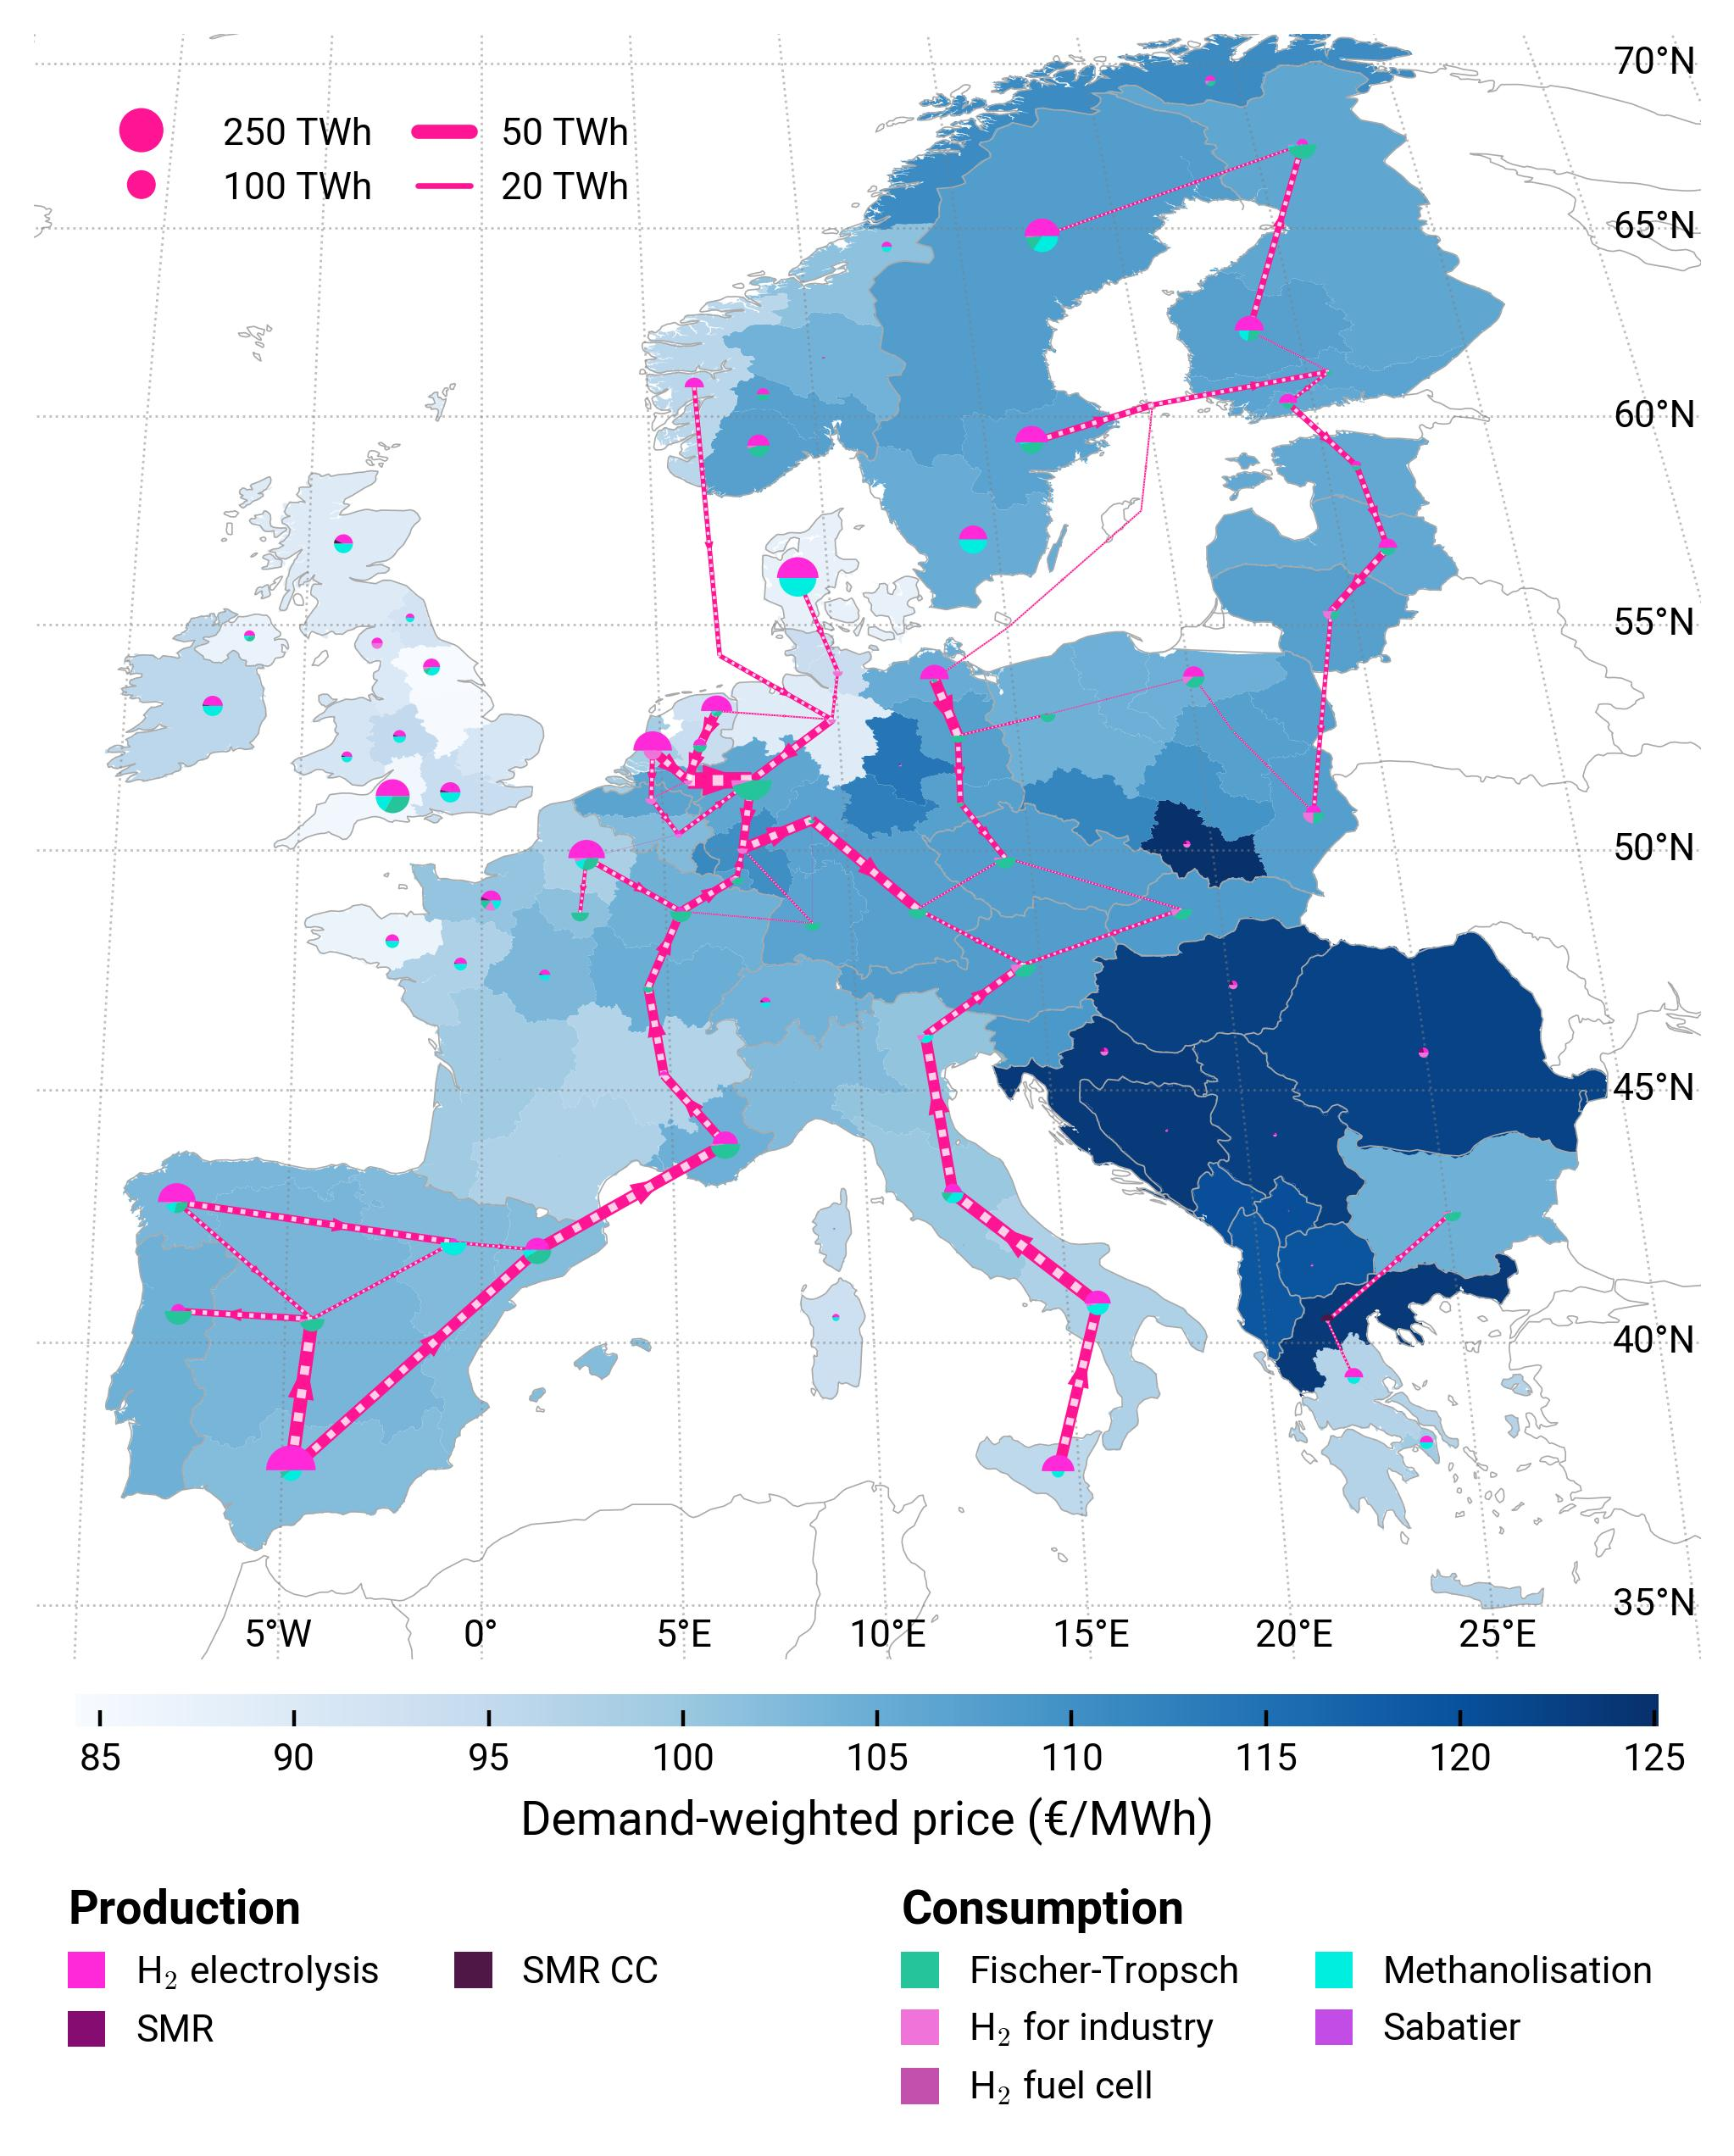
\includegraphics[width=0.8\textwidth]{maps/pcipmi/base_s_adm___2040-balance_map_H2}
%       \end{figure}
%     \end{column}
%     \begin{column}{0.5\textwidth}
%       \begin{figure}
%         \centering
%         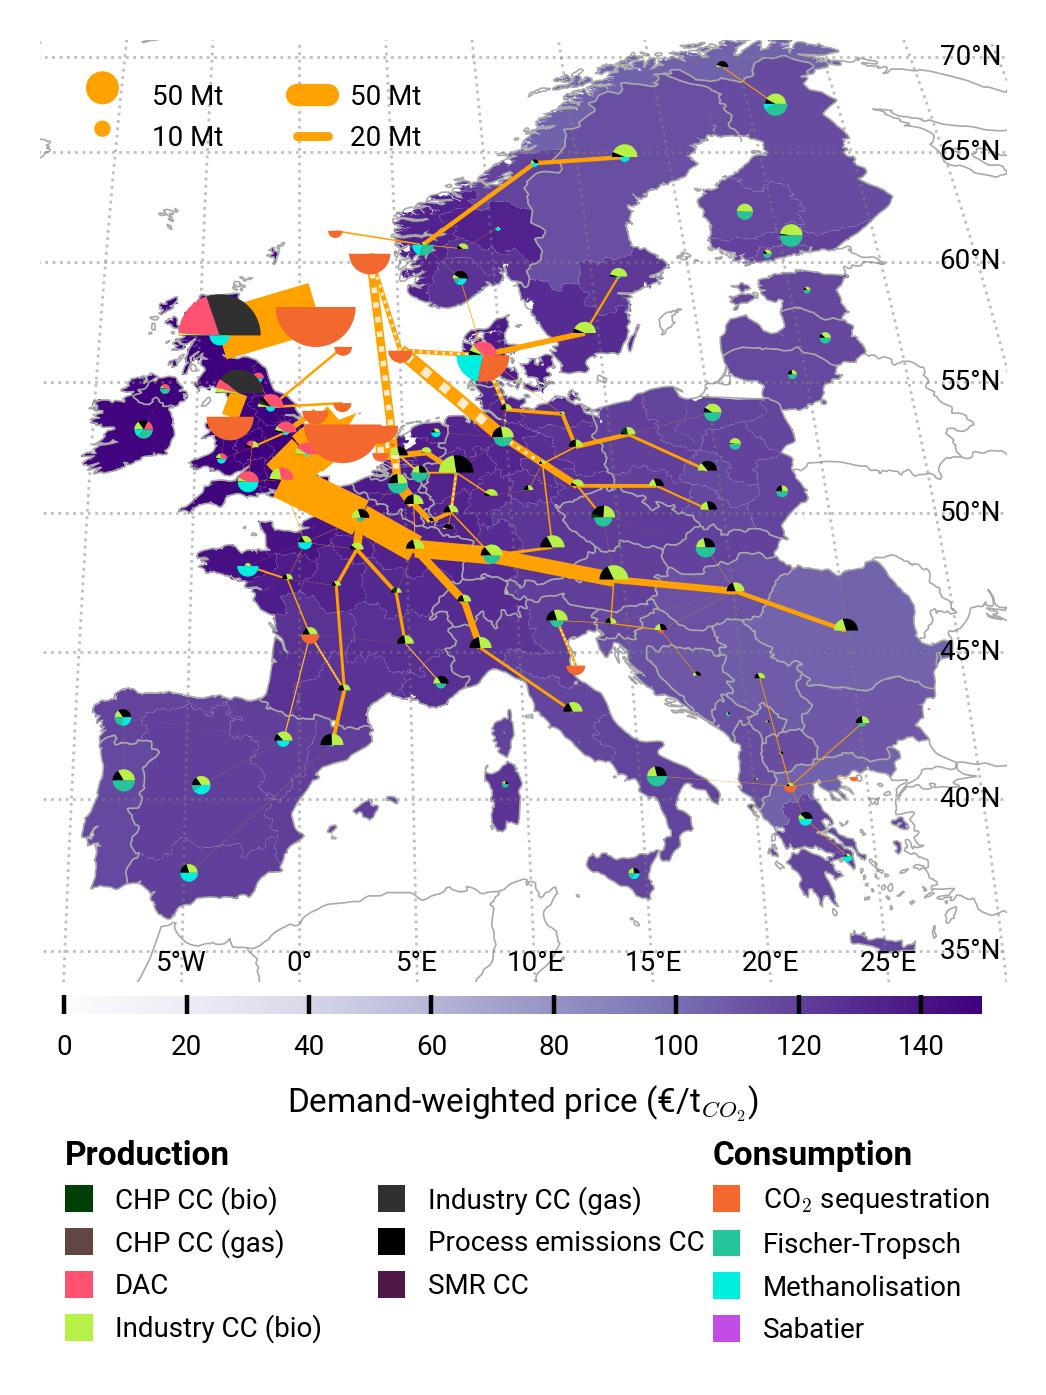
\includegraphics[width=0.8\textwidth]{maps/pcipmi/base_s_adm___2040-balance_map_co2_stored}
%       \end{figure}
%     \end{column}
%   \end{columns}
%   \source{Own illustration.}
% \end{frame}

\begin{frame}{LT --- PCI: 2050 regional \ce{H2}, \ce{CO2} balances and transport}
  \centering
  \begin{columns}
    \begin{column}{0.5\textwidth}
      \footnotesize
      \begin{figure}
        \centering
        \includegraphics[width=0.8\textwidth]{maps/pcipmi/base_s_adm___2050-balance_map_H2}
      \end{figure}
    \end{column}
    \begin{column}{0.5\textwidth}
      \begin{figure}
        \centering
        \includegraphics[width=0.8\textwidth]{maps/pcipmi/base_s_adm___2050-balance_map_co2_stored}
      \end{figure}
    \end{column}
  \end{columns}
  \source{Own illustration.}
\end{frame}

\begin{frame}{LT --- \ce{CO2} balances}
  \centering
  \begin{columns}
    \begin{column}{0.48\textwidth}
      \footnotesize
      \begin{figure}
        \centering
        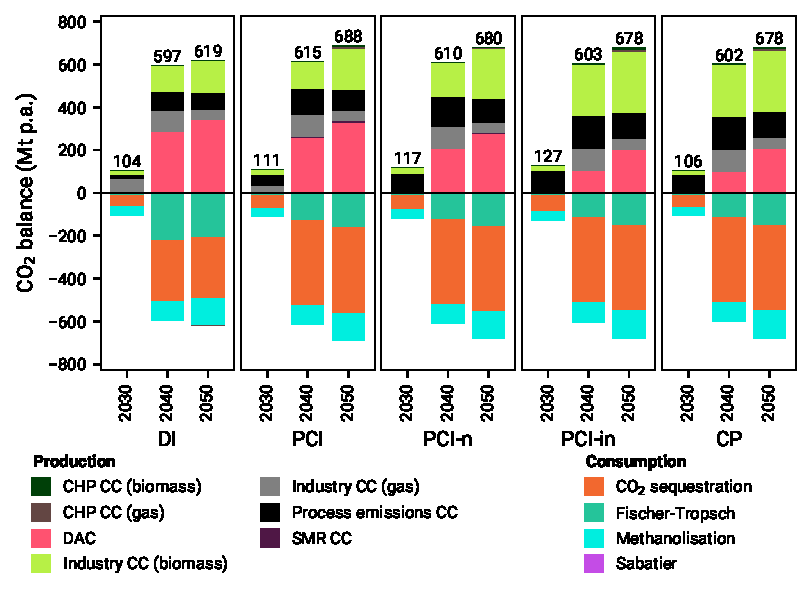
\includegraphics[width=1\textwidth]{balances_overview_co2 stored}
      \end{figure}
    \end{column}
    \begin{column}{0.52\textwidth}
      \footnotesize
      \begin{itemize}
        \item With increasing pipeline build-out to transport \ce{CO2} from industry and other point sources to sequestration sites, DAA utilisation decreases by almost half (left to right)
        \item In 2030, 50 Mt p.a. sequestration target is binding, if no pipelines are built. With pipeline build-out, up to 75 Mt p.a. are sequestered
        \item In 2040 and 2050, all sequestration targets are overachieved, potential of 398 Mt p.a. is fully exploited in all scenarios with PCI-PMI projects.
        \item Biomass-based industry contributing the largest share of point-source carbon capture
        \item With lower sequestration potential of 386 Mt p.a. in \textit{DI} scenario, more \ce{CO2} goes into carbon utilisation (Fischer-Tropsch synthesis) instead
      \end{itemize}
    \end{column}
  \end{columns}
  \source{Own illustration.}
\end{frame}

\begin{frame}{LT --- \ce{CO2} balances: Direct Air Capture utilisation}
  \begin{figure}[htbp]
    \centering
    \includegraphics[width=0.75\textwidth]{delta_balances_dac}
  \end{figure}
\end{frame}

\begin{frame}{LT --- \ce{H2} balances}
  \centering
  \begin{columns}
    \begin{column}{0.48\textwidth}
      \footnotesize
      \begin{figure}
        \centering
        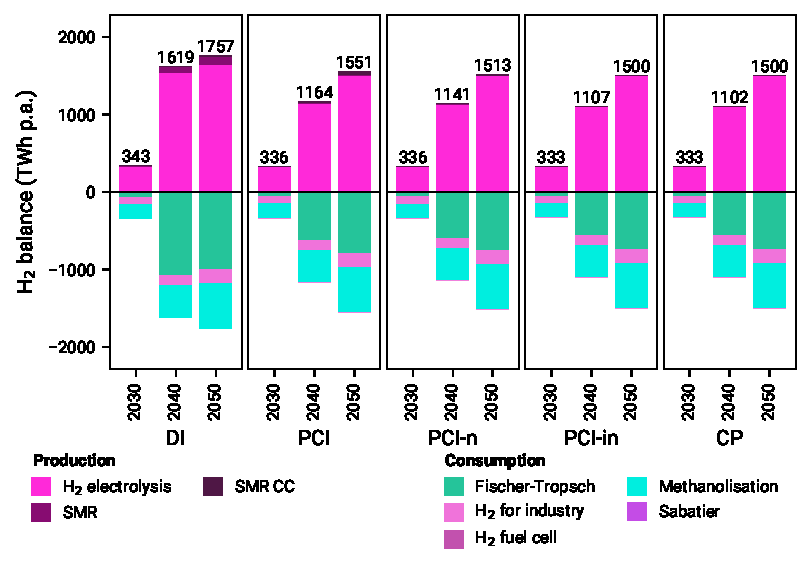
\includegraphics[width=1\textwidth]{balances_overview_H2}
      \end{figure}
    \end{column}
    \begin{column}{0.52\textwidth}
      \footnotesize
      \begin{itemize}
        \item \ce{H2} production primarily driven by demand for Fischer-Tropsch fuels and methanol
        \item In 2050, Fischer-Tropsch fuels primarily used to satisfy kerosene in aviation and industrial naphta
        \item When no pipelines are built, \ce{H2} production is significantly higher, given the need for additional Fischer-Tropsch synthesis to bind \ce{CO2} as an alternative to sequestration
        \item \ce{H2} 71 to 102 TWh p.a. from Steam Methane Reforming without pipelines.
      \end{itemize}
    \end{column}
  \end{columns}
  \source{Own illustration.}
\end{frame}

\begin{frame}{Regret analysis}
  \centering
  \begin{columns}
  \begin{column}{0.4\textwidth}
      \footnotesize
      \begin{itemize}
        \item Regret is calculated by subtracting annual total system costs of long-term from short-term scenarios
        \item Regret terms represent additional cost incurred by given short-term incident relative to benchmark scenario
        \item Positive values indicate higher costs, driven by increased investments into alternative generation, conversion, storage, and CDR technologies, as well as changes in their operation
        \item Negative values indicate cost savings, which may arise under relaxed policy ambitions 
      \end{itemize}
    \end{column}
    \begin{column}{0.6\textwidth}
      \footnotesize
      \begin{figure}
        \centering
        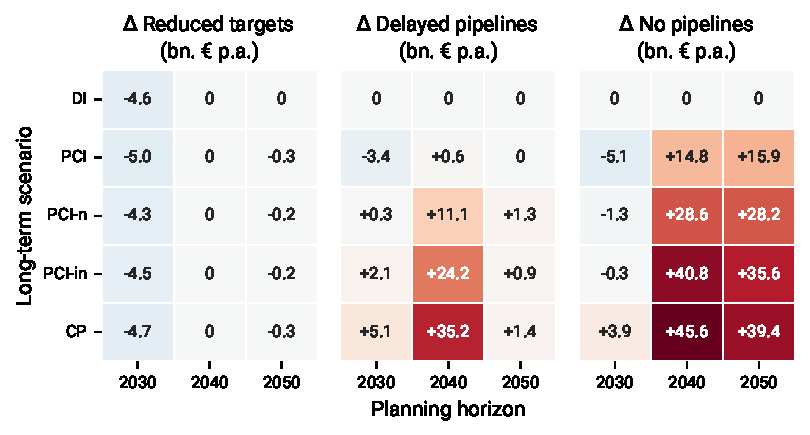
\includegraphics[width=1\textwidth]{regret_matrix}
      \end{figure}
    \end{column}
  \end{columns}
  \source{Own illustration.}
\end{frame}

\begin{frame}{Value of PCI-PMI projects in the long run}
  \begin{figure}[htbp]
    \centering
    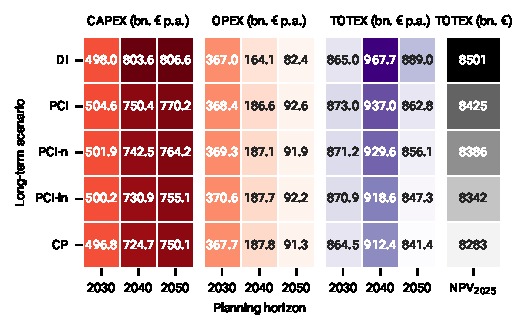
\includegraphics[width=0.65\textwidth]{totex_heatmap}
  \end{figure}
\end{frame}

\section{Conclusion}

\begin{frame}{Conclusion}
\vspace{-0.4cm}
\begin{columns}[t,onlytextwidth]
  \footnotesize
  \column{0.49\textwidth}
    \begin{tcolorbox}[colback=blue!5, colframe=blue!40!black, fonttitle=\bfseries, title=Economic viability \& policy targets]
    \centering
    \scriptsize
    \begin{itemize}
      \item PCI-PMI pipelines bring net system cost reductions, visible in the long-run
      \item Strategic extensions amplify benefits  
      \item Support EU GHG reduction, H\textsubscript{2}, and CO\textsubscript{2} sequestration targets  
      \item Low-regret investment, even when accounting for delays
    \end{itemize}
    \end{tcolorbox}
    
    \vspace{0.02cm}
    \begin{tcolorbox}[colback=orange!5, colframe=orange!60!black, fonttitle=\bfseries, title=Tech \& risk diversification]
    \centering
    \scriptsize
    \begin{itemize}
      \item Pipelines boost more efficient use from RES  
      \item Reduce reliance on point source CC and costly, low-TRL CDR technologies, such as DAC  
    \end{itemize}
    \end{tcolorbox}

  \column{0.49\textwidth}
    \begin{tcolorbox}[colback=green!5, colframe=green!40!black, fonttitle=\bfseries, title=CCUS \& hydrogen utilisation]
    \centering
    \scriptsize
    \begin{itemize}
      \item Dual purpose: \ce{H2} pipelines link high RES regions to demand centers while \ce{CO2} pipelines connect industry to sequestration sites  
      \item Enable decarbonisation of hard-to-abate sectors and industrial processing including non-abatle process emissions
    \end{itemize}
    \end{tcolorbox}
    
    \vspace{-0.2cm}
    
    \begin{tcolorbox}[colback=red!5, colframe=red!50!black, fonttitle=\bfseries, title=Political support \& acceptance]
    \centering
    \scriptsize
     \begin{itemize}
      \item EU backing ensures funding \& fast permitting  
      \item Frequent reporting \& transparency builds public trust and acceptance
      \item Advantage over purely cost-optimal, theoretical plans
    \end{itemize}
    \end{tcolorbox}
\end{columns}
\end{frame}

% \begin{frame}{Conclusion}
%   \footnotesize
%   \begin{enumerate}
%     \setlength\itemsep{0.3em}
%     \item PCI-PMI projects have a positive impact on total system costs and are likely a no-regret investment based on our results (though not perfectly cost-optimal compared to theoretical \textit{CP} scenario).
%     \item Additional cost savings can be unlocked with single, strategically placed pipelines to connect additional \ce{H2} production sites and \ce{CO2} point sources to the pipeline network.
%     \item Further, the success of large-scale investment projects is largely driven by political support, public acceptance, which is especially given for PCI-PMI projects.
%     \item \ce{H2} pipelines projects help distribute more affordable green H$_2$ from northern and south-western Europe to high-demand regions in central Europe; ii) \ce{CO2} transport and storage projects help decarbonising the industry by connecting major industrial sites and their process emissions to offshore sequestration sites in the North Sea (Denmark, Norway, and the Netherlands).
%     \item Pipelines basically serve as a tool to hedge risks of overbuilding solar and wind generation capacities and reduce excessive reliance on single carbon capture technologies like DAC and carbon capture at point sources $\rightarrow$ confirms previous findings of \cite{hofmannH2CO2Network2025}.
%     \item Overall, PCI-PMI projects including additional pipeline build-outs allow a lower-cost and less technology-dependent transition towards a decarbonised system compared to a system without any pipeline infrastructure. They support achieving the EUs ambitious policy targets in the long run.
%   \end{enumerate}

% \end{frame}


% \begin{frame}[allowframebreaks]{References (excerpt)}
\begin{frame}{References (excerpt)}
  \begingroup
  \renewcommand*{\bibfont}{\scriptsize}
  \printbibliography
  \endgroup
\end{frame}

\begin{frame}
  \setbeamercolor{background canvas}{bg=red}
  \centering
  \fcolorbox{white}{tub-red}{\parbox[c][0.9\textheight][c]{\textwidth}{%
      \centering \color{white}\Large{\textbf{Thank you.}} \\ 
      \scriptsize
      \vspace{0.5cm}
      \href{https://github.com/pypsa/pypsa-eur}{\textcolor{white}{$\hookrightarrow$ github.com/pypsa/pypsa-eur}} \\
      \vspace{0.5cm}
      Department of\\\textbf{Digital Transformation in Energy Systems (ENSYS)} \\
      \vspace{0.5cm}
      \textbf{Bobby Xiong}\\
      \href{mailto:xiong@tu-berlin.de}{\textcolor{white}{$\hookrightarrow$ xiong@tu-berlin.de}} \\
      \href{https://github.com/bobbyxng}{\textcolor{white}{$\hookrightarrow$ github.com/bobbyxng}} \\
  }}
\end{frame}

% Appendix
\section{Appendix}

\begin{frame}
  \setbeamercolor{background canvas}{bg=red}
  \centering
  \fcolorbox{white}{tub-red}{\parbox[c][0.9\textheight][c]{\textwidth}{%
      \centering \color{white}\Large{\textbf{Appendix}}
  }}
\end{frame}

\begin{frame}{Cost assumptions for key technologies}
  \scriptsize
  \centering
  \begin{tabularx}{0.8\textwidth}{R{2.4cm}>{\centering\arraybackslash}X>{\centering\arraybackslash}X>
  {\centering\arraybackslash}X}
    \toprule
    & \textbf{Unit} & \textbf{CAPEX} & \textbf{FOM} \\
    \midrule
    \textbf{\ce{Pipeline infrastructure}} & & & \\
    \ce{CO2} onshore pipelines & \euro{}/t\ce{CO2}/hkm & \num{2116} & \SI{0.9}{\percent/a} \\
    \ce{CO2} offshore pipelines & \euro{}/t\ce{CO2}/hkm & \num{4233} & \SI{0.5}{\percent/a} \\
    \ce{H2} onshore pipelines & \euro{}/MW$_{H_2}$/km & \num{304} & 1.5-\SI{3.2}{\percent/a} \\
    \ce{H2} offshore pipelines & \euro{}/MW$_{H_2}$/km & \num{456} & \SI{3.0}{\percent/a} \\
    \midrule
    \textbf{\ce{Conversion}} & & & \\
    Electrolysis & \euro{}/kW$_e$ & \num{1000}-\num{1500} & \SI{4.0}{\percent/a} \\
    SMR & \euro{}/MW$_{CH_4}$ & \num{522201} & \SI{5.0}{\percent/a} \\
    SMR CC & \euro{}/MW$_{CH_4}$ & \num{605753} & \SI{5.0}{\percent/a} \\

    \bottomrule
  \end{tabularx}
  \source{Own illustration.}

\end{frame}

\begin{frame}{LT --- Installed capacities}
  \begin{figure}[htbp]
    \centering
    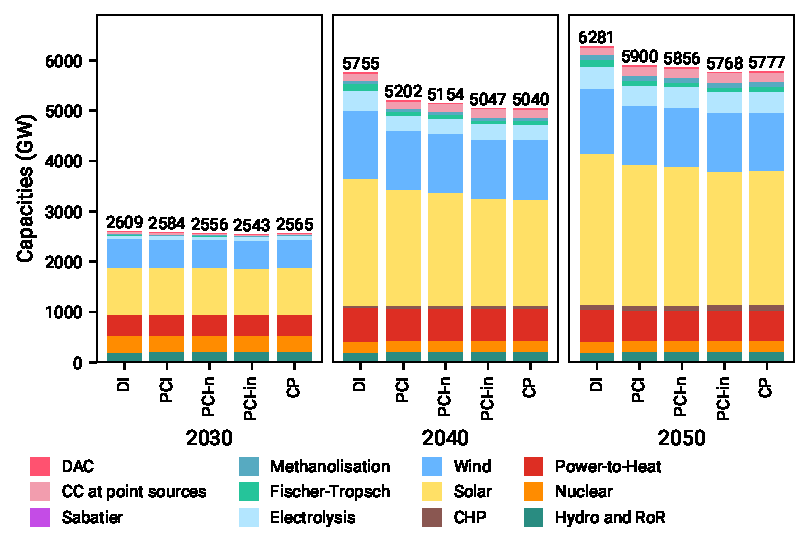
\includegraphics[width=0.65\textwidth]{capacities_overview}
  \end{figure}
\end{frame}

\begin{frame}{ST --- Delta system costs}
  \begin{figure}[htbp]
    \centering
    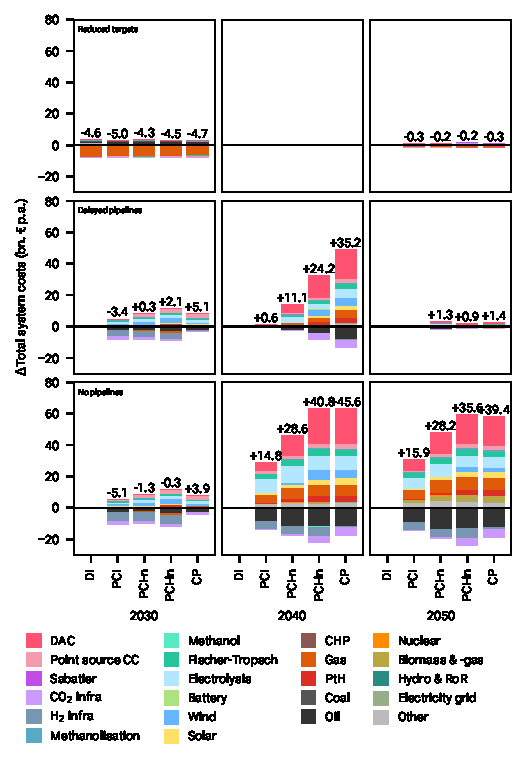
\includegraphics[width=0.36\textwidth]{costs_overview_extended}
  \end{figure}
\end{frame}

\begin{frame}{ST --- Delta capacities}
  \begin{figure}[htbp]
    \centering
    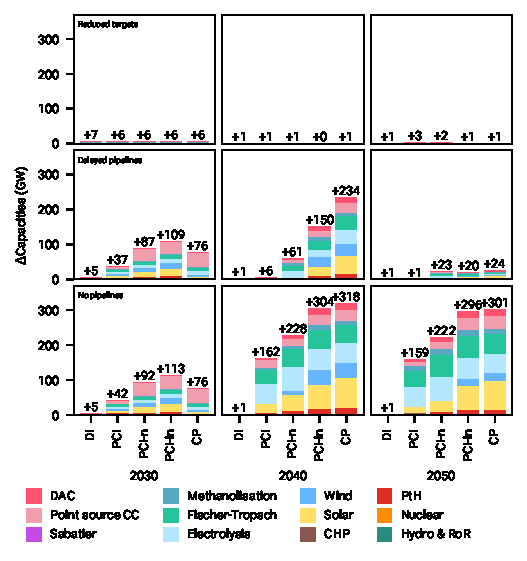
\includegraphics[width=0.45\textwidth]{capacities_overview_extended}
  \end{figure}
\end{frame}

\begin{frame}{ST --- Delta balances \ce{CO2}}
  \begin{figure}[htbp]
    \centering
    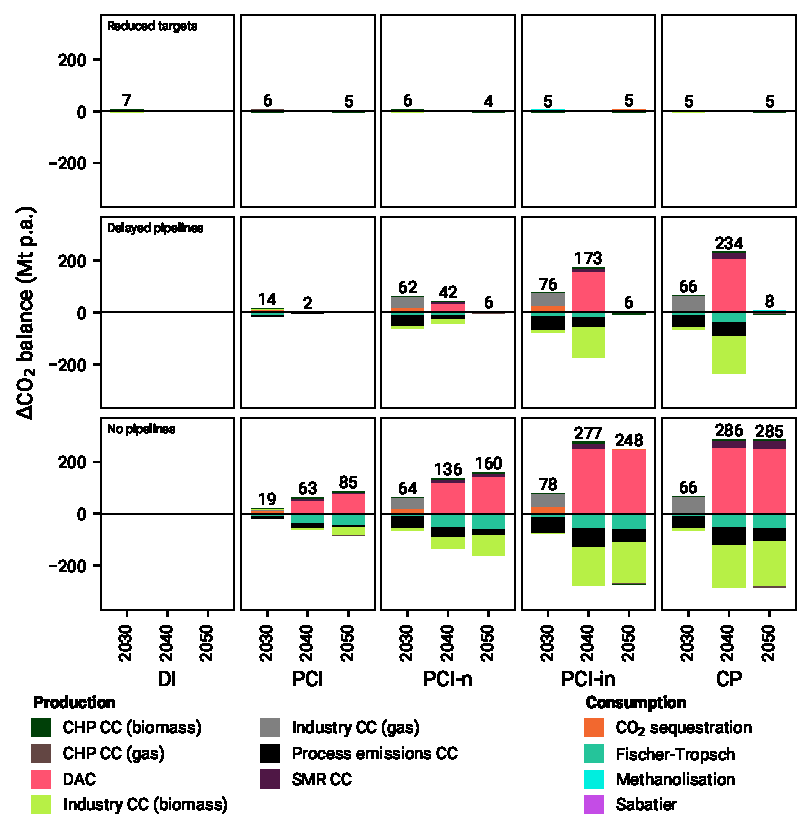
\includegraphics[width=0.44\textwidth]{balances_overview_extended_co2 stored}
  \end{figure}
\end{frame}

\begin{frame}{ST --- Delta balances \ce{H2}}
  \begin{figure}[htbp]
    \centering
    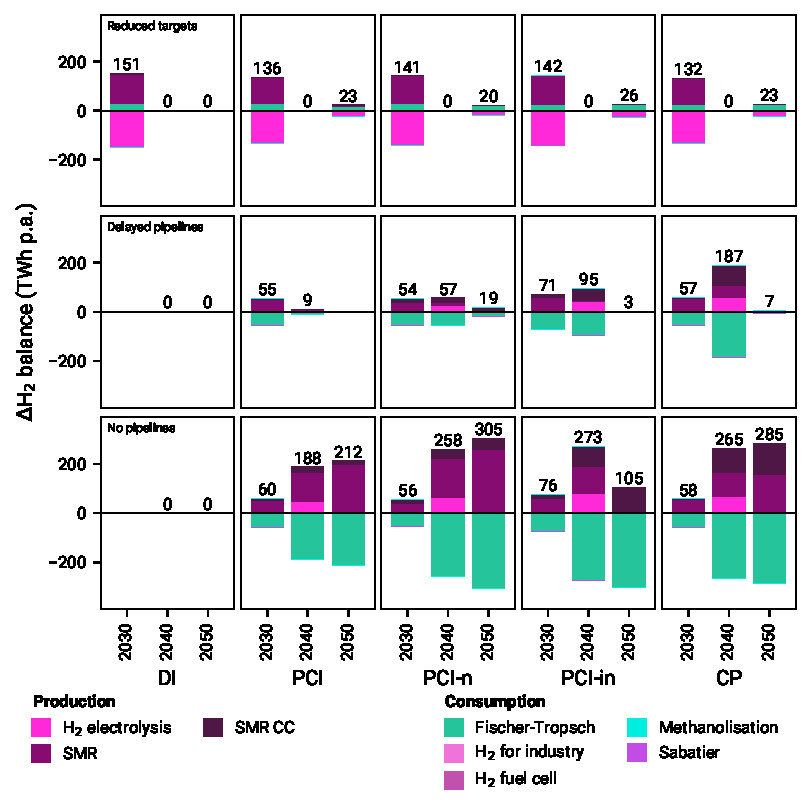
\includegraphics[width=0.45\textwidth]{balances_overview_extended_H2}
  \end{figure}
\end{frame}

\begin{frame}{DI --- PCI: 2050 regional \ce{H2}, \ce{CO2} balances, transport, and prices}
  \centering
  \begin{columns}
    \begin{column}{0.5\textwidth}
      \footnotesize
      \begin{figure}
        \centering
        \includegraphics[width=0.76\textwidth]{maps/no-pipelines-no-pcipmi/base_s_adm___2050-balance_map_H2}
      \end{figure}
    \end{column}
    \begin{column}{0.5\textwidth}
      \begin{figure}
        \centering
        \includegraphics[width=0.76\textwidth]{maps/no-pipelines-no-pcipmi/base_s_adm___2050-balance_map_co2_stored}
      \end{figure}
    \end{column}
  \end{columns}
  \source{Own illustration.}
\end{frame}

\begin{frame}{PCI-n --- PCI: 2050 regional \ce{H2}, \ce{CO2} balances, transport, and prices}
  \centering
  \begin{columns}
    \begin{column}{0.5\textwidth}
      \footnotesize
      \begin{figure}
        \centering
        \includegraphics[width=0.76\textwidth]{maps/pcipmi-national-expansion/base_s_adm___2050-balance_map_H2}
      \end{figure}
    \end{column}
    \begin{column}{0.5\textwidth}
      \begin{figure}
        \centering
        \includegraphics[width=0.76\textwidth]{maps/pcipmi-national-expansion/base_s_adm___2050-balance_map_co2_stored}
      \end{figure}
    \end{column}
  \end{columns}
  \source{Own illustration.}
\end{frame}

\begin{frame}{PCI-in --- PCI: 2050 regional \ce{H2}, \ce{CO2} balances, transport, and prices}
  \centering
  \begin{columns}
    \begin{column}{0.5\textwidth}
      \footnotesize
      \begin{figure}
        \centering
        \includegraphics[width=0.76\textwidth]{maps/pcipmi-national-international-expansion/base_s_adm___2050-balance_map_H2}
      \end{figure}
    \end{column}
    \begin{column}{0.5\textwidth}
      \begin{figure}
        \centering
        \includegraphics[width=0.76\textwidth]{maps/pcipmi-national-international-expansion/base_s_adm___2050-balance_map_co2_stored}
      \end{figure}
    \end{column}
  \end{columns}
  \source{Own illustration.}
\end{frame}

\begin{frame}{CP --- PCI: 2050 regional \ce{H2}, \ce{CO2} balances, transport, and prices}
  \centering
  \begin{columns}
    \begin{column}{0.5\textwidth}
      \footnotesize
      \begin{figure}
        \centering
        \includegraphics[width=0.76\textwidth]{maps/greenfield-pipelines/base_s_adm___2050-balance_map_H2}
      \end{figure}
    \end{column}
    \begin{column}{0.5\textwidth}
      \begin{figure}
        \centering
        \includegraphics[width=0.76\textwidth]{maps/greenfield-pipelines/base_s_adm___2050-balance_map_co2_stored}
      \end{figure}
    \end{column}
  \end{columns}
  \source{Own illustration.}
\end{frame}

\begin{frame}{\textbf{Why H$_2$?} Most H$_2$ is used for derivative fuels and chemicals!}
  
  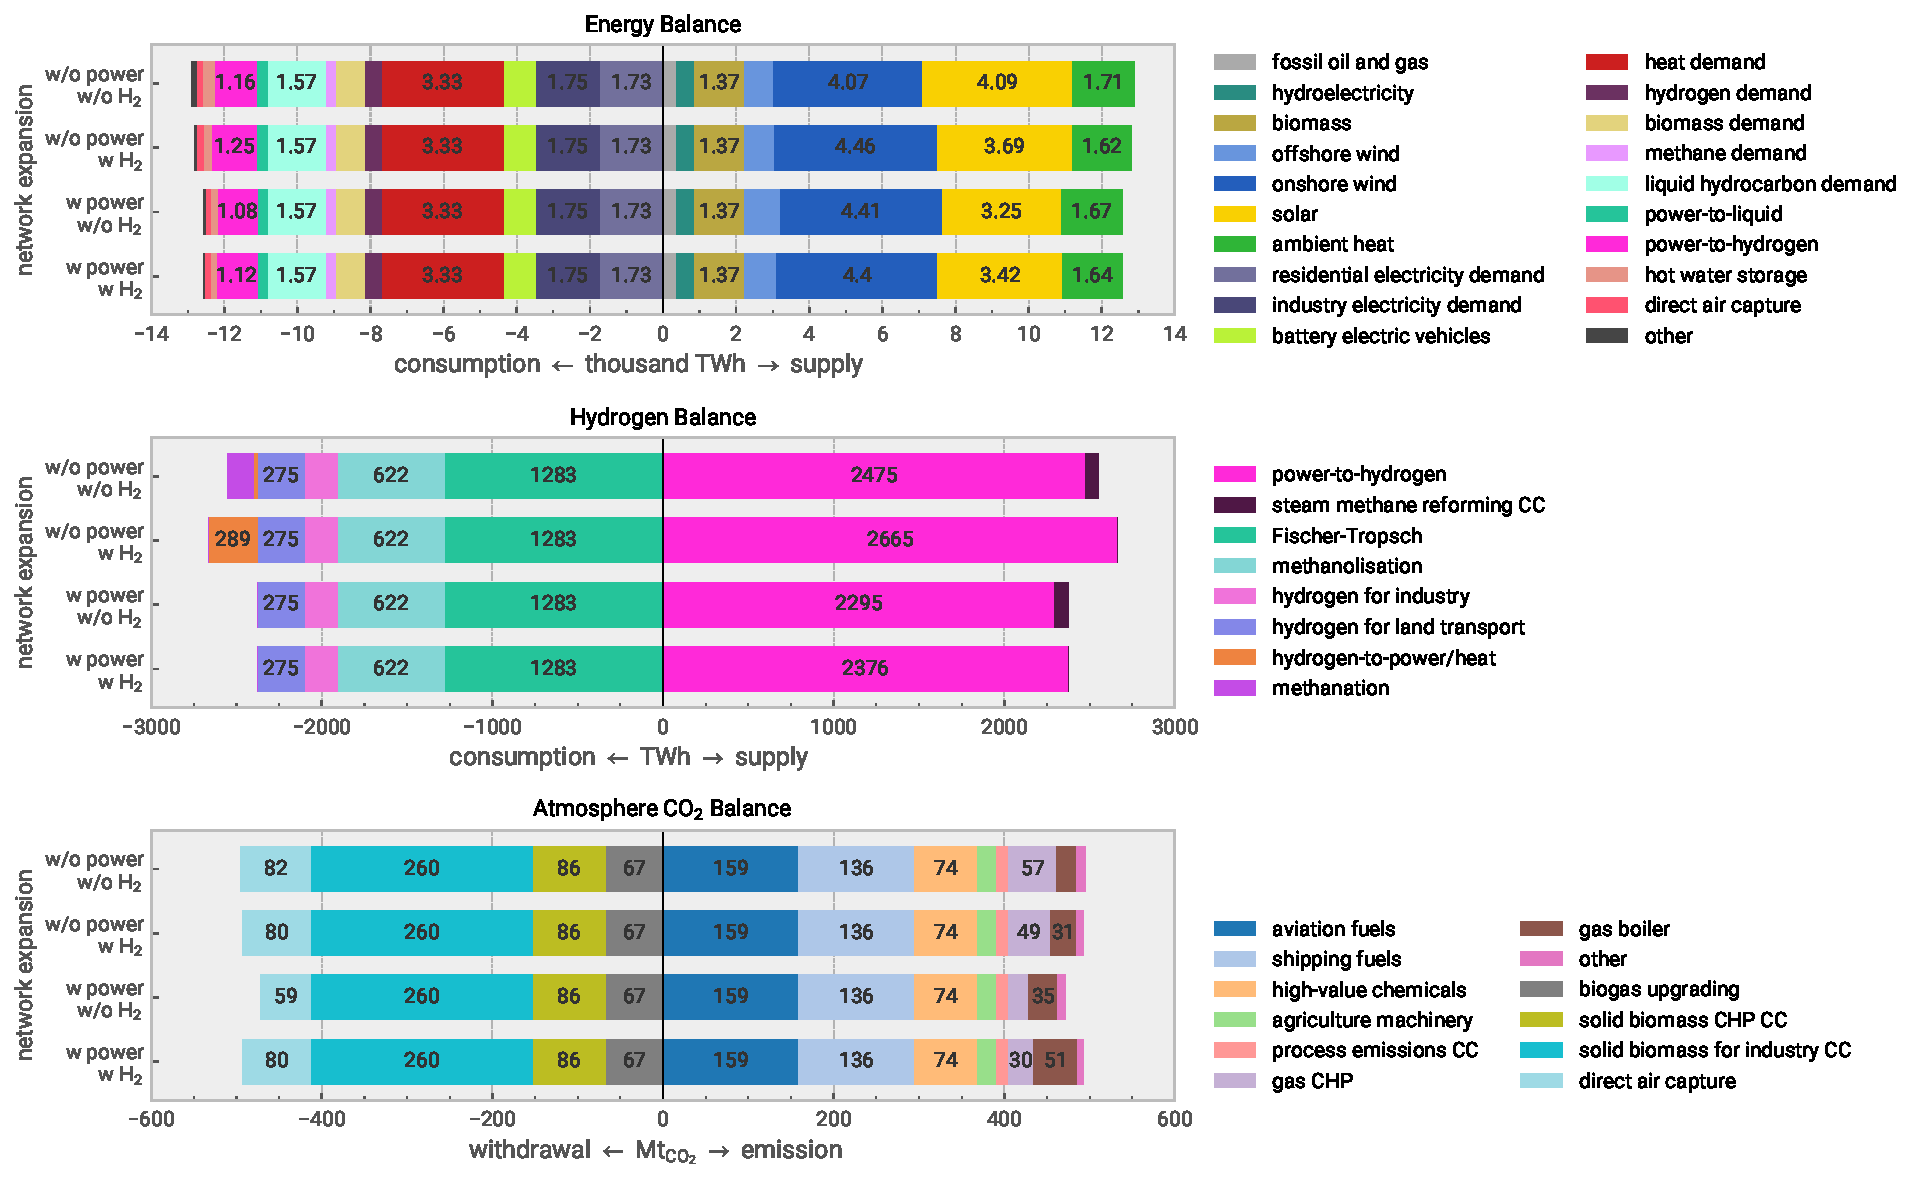
\includegraphics[width=1.2\textwidth, trim=0cm 6.6cm 0cm 6.6cm, clip]{other/hydrogen_balance.pdf}

  \footnotesize

  Mostly \alert{green electrolytic hydrogen supply}. \alert{Few direct uses of hydrogen} in the energy system, but it is
  used to synthesise other fuels and chemicals:

  \begin{multicols}{2}
  \begin{itemize}
    \item ammonia for fertilizers
    \item direct reduced iron for steelmaking
    \item shipping and aviation fuels
    \item precursor to high-value chemicals
    \item backup heat and power supply
    \item some heavy duty land transport
  \end{itemize}
  \end{multicols}

  \source{Neumann, Zeyen, Victoria, Brown, 2023\\\url{https://doi.org/10.1016/j.joule.2023.06.016}}
\end{frame}

\begin{frame}{Transporting \textbf{CO$_2$ to H$_2$} or transporting \textbf{H$_2$ to CO$_2$}?}
  
  \centering
  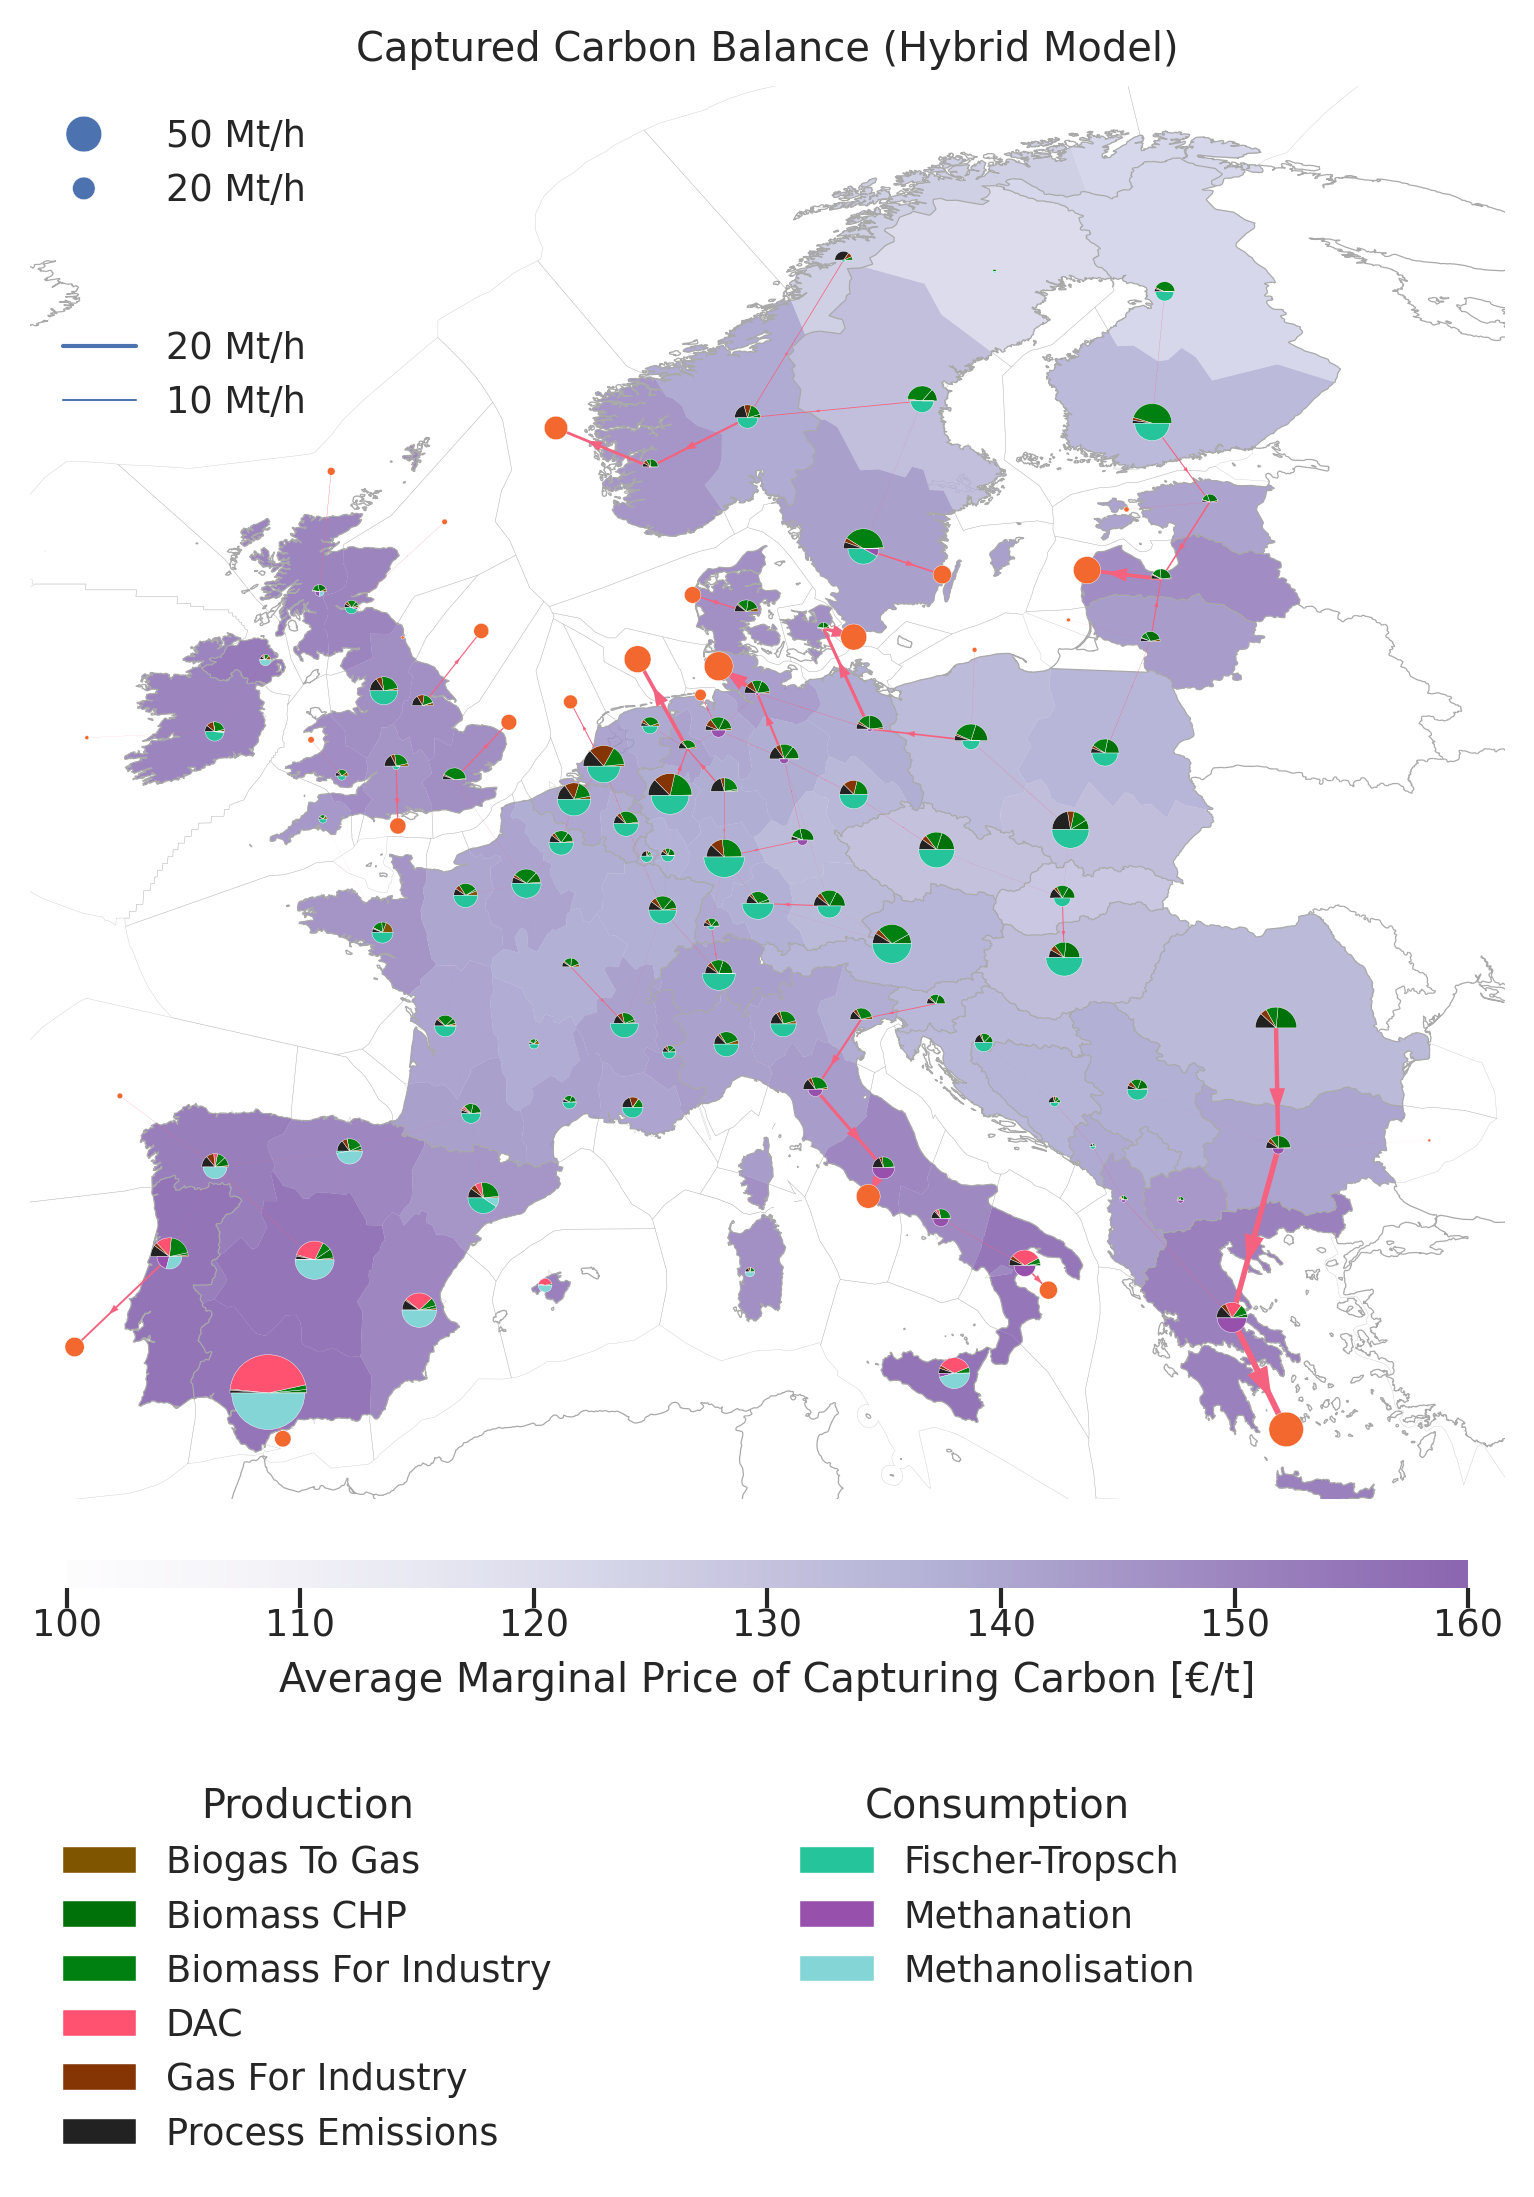
\includegraphics[width=0.35\textwidth]{other/carbon_networks_balance_map_carbon}
  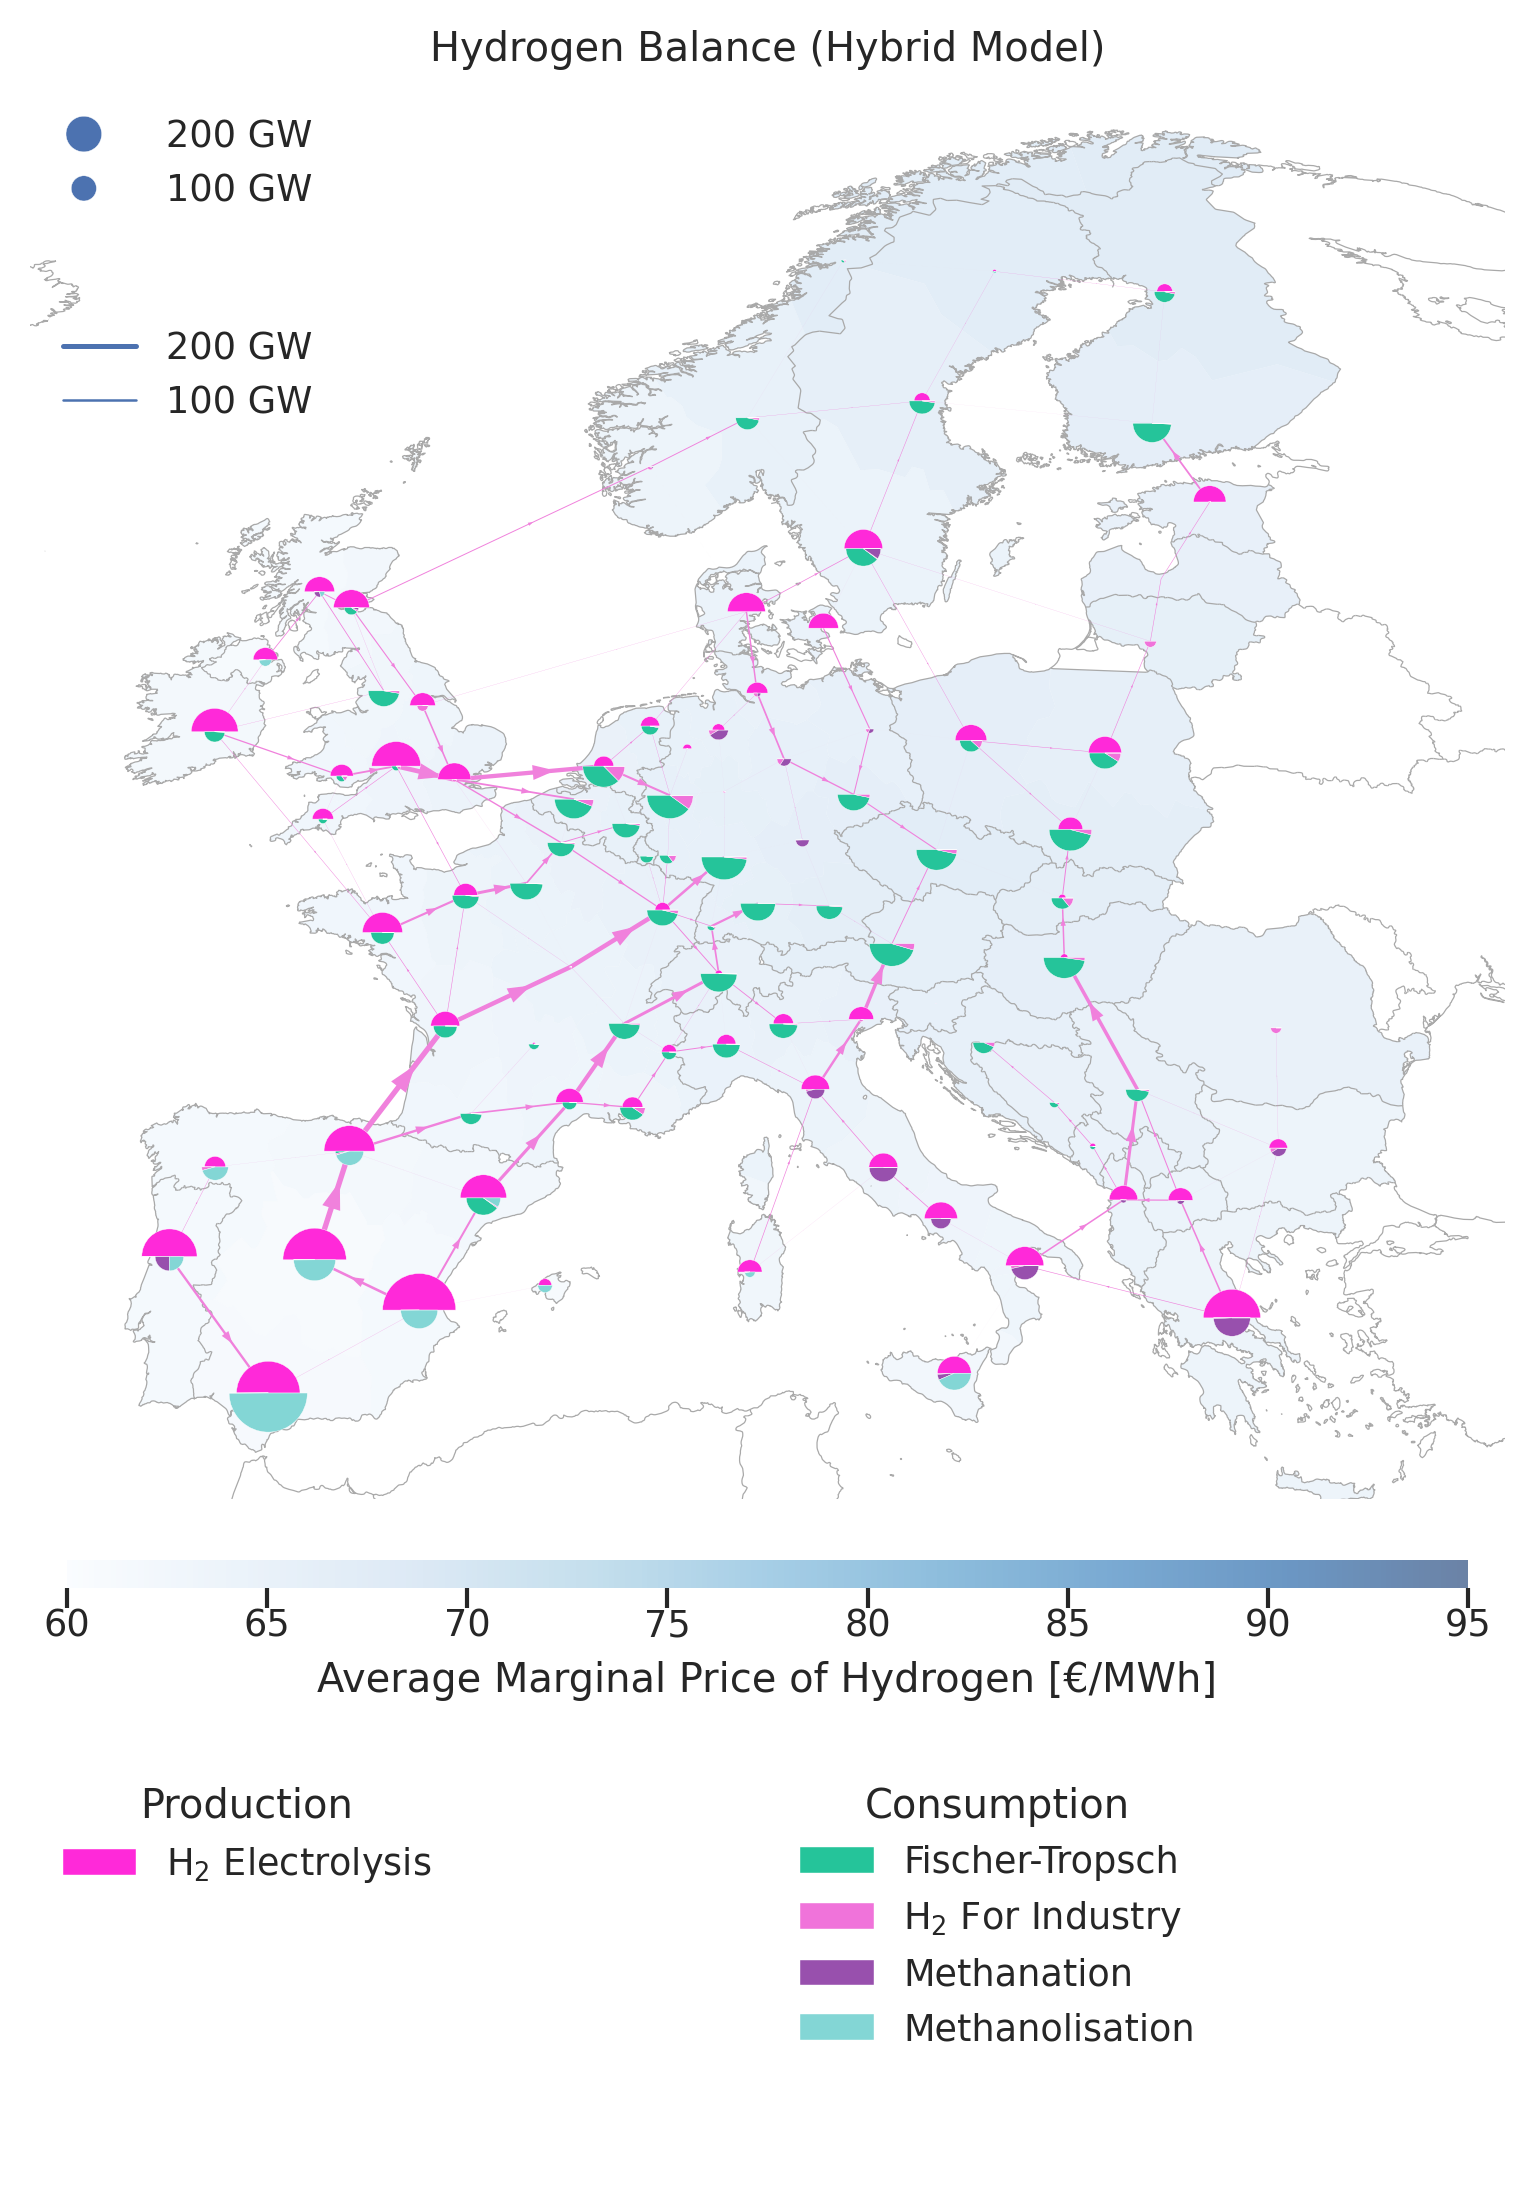
\includegraphics[width=0.35\textwidth]{other/carbon_networks_balance_map_hydrogen}

  \source{Hofmann, Tries, Neumann, Zeyen, Brown, 2024\\\url{https://arxiv.org/abs/2402.19042}}

\end{frame}


\begin{frame}{\textbf{Carbon management}: Capture, use, transport and sequestration}
  
  \begin{center}
    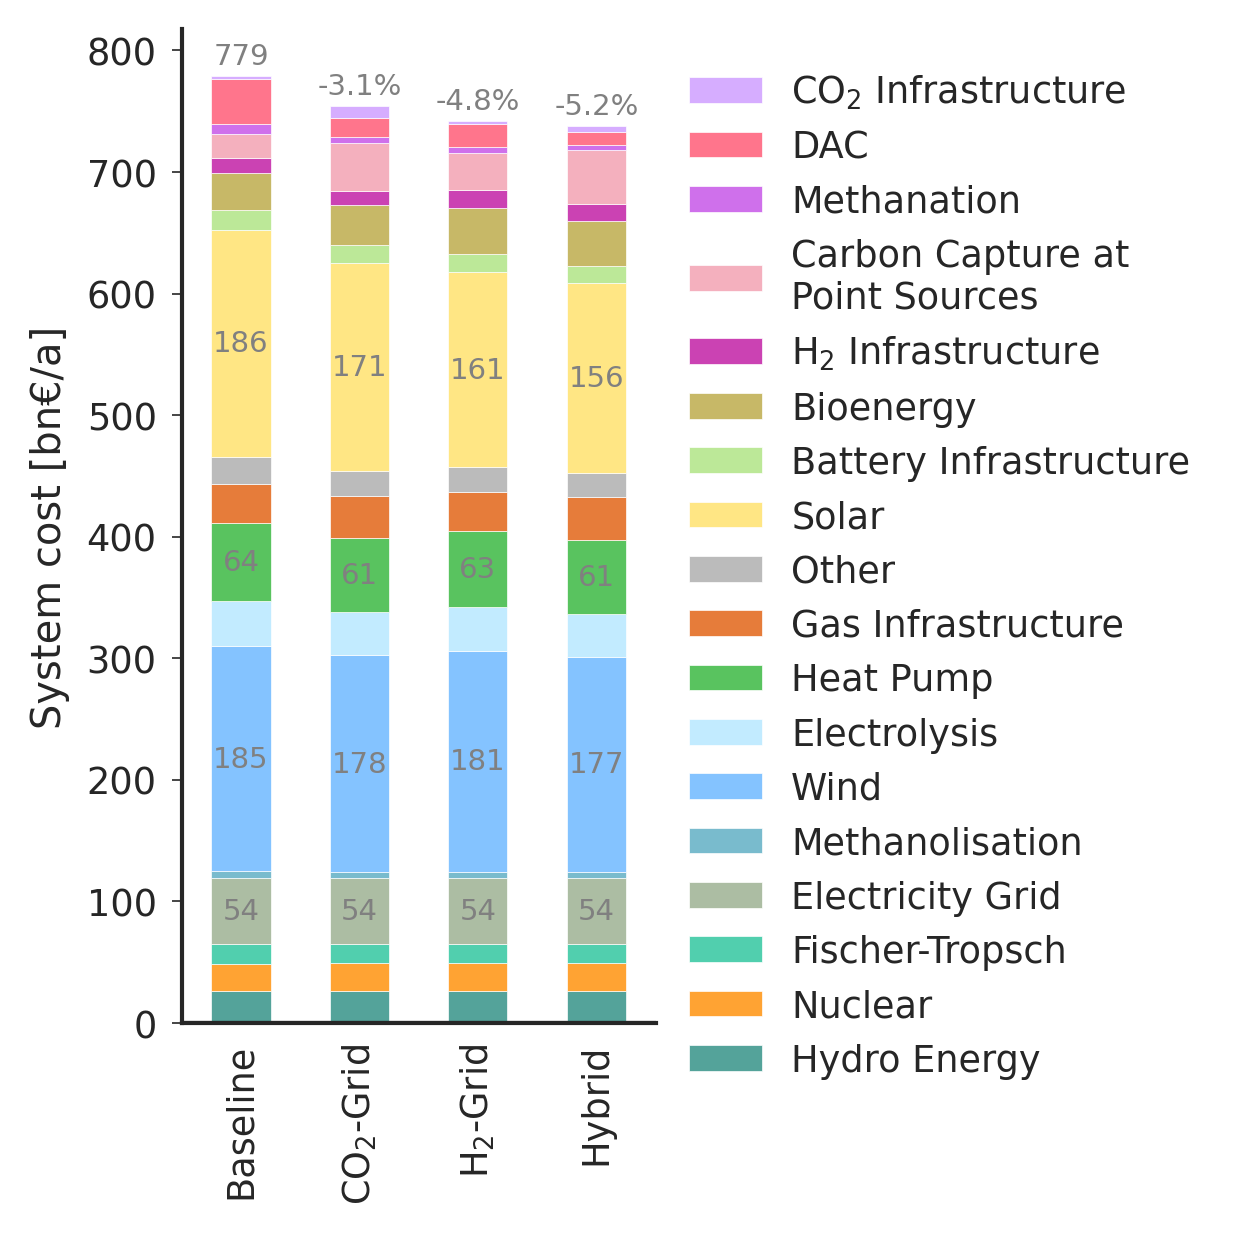
\includegraphics[height=0.73\textheight]{other/carbon_networks_cost_bar}
    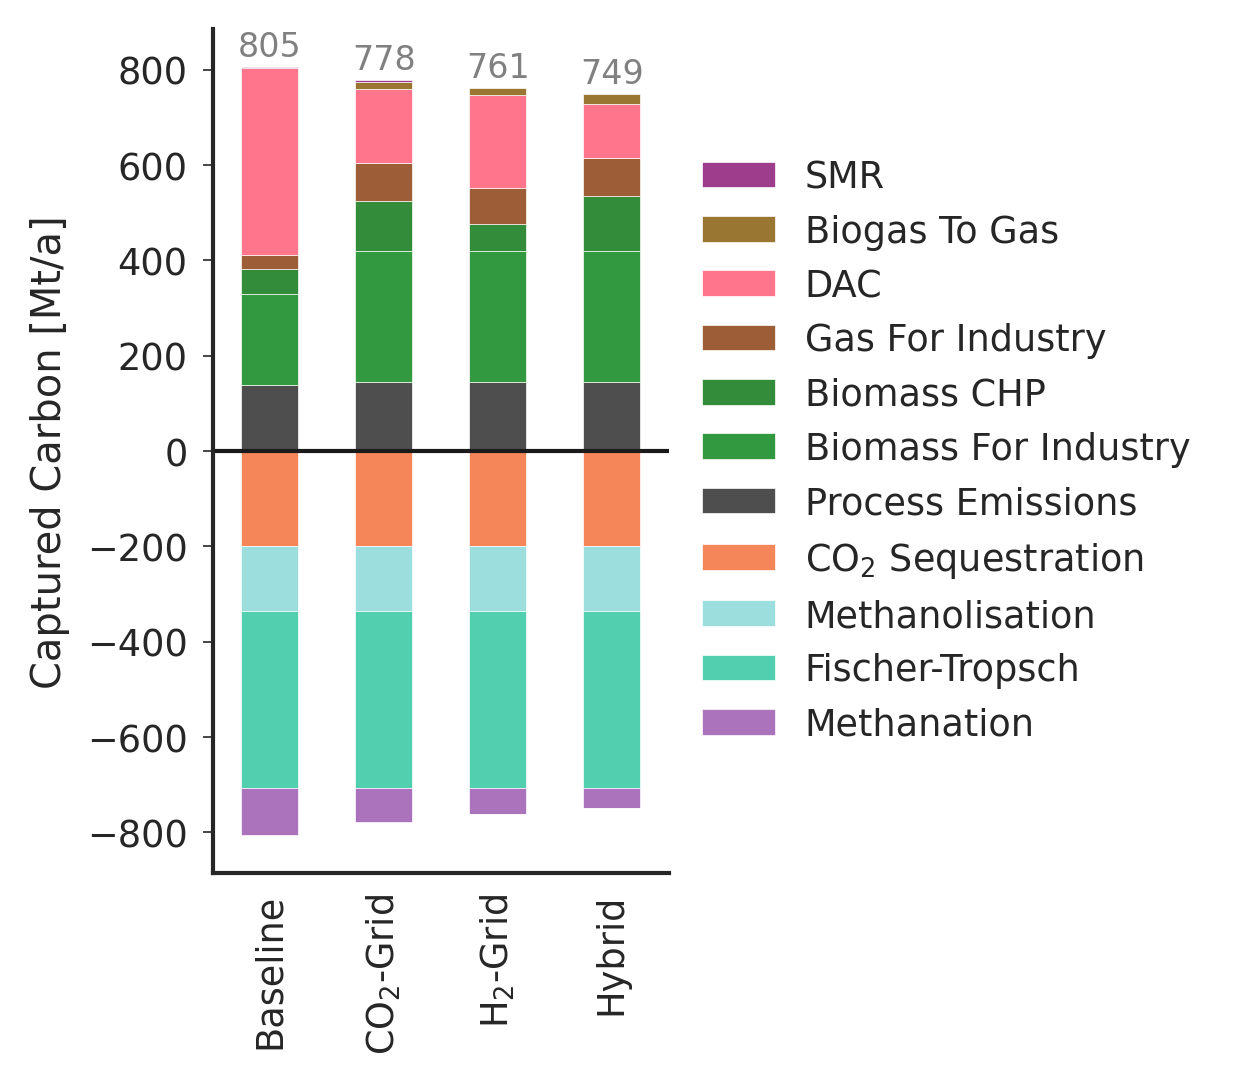
\includegraphics[height=0.71\textheight]{other/carbon_networks_balance_bar_carbon}

    \vspace{-0.25cm}
    \footnotesize
    \begin{itemize}
      \item \alert{CCS} for process emissions (for instance, in cement industry)
      \item \alert{CCU} for e-synfuels and e-chemicals (in particular, shipping, aviation, plastics)
      \item \alert{CDR} for unabatable and negative emissions (to offset imperfect capture rates)
    \end{itemize}

  \end{center}

  \source{Hofmann, Tries, Neumann, Zeyen, Brown, 2024\\\url{https://arxiv.org/abs/2402.19042}}

\end{frame}

\begin{frame}{Electricity high-voltage grid based on OpenStreetMap (OSM)}

  \begin{columns}
    \begin{column}{0.64\textwidth}
      \footnotesize
      \begin{itemize}
        \setlength\itemsep{.8em}
        \item Dataset contains a topologically connected representation of the European high-voltage grid (220 kV to 750 kV) constructed using OpenStreetMap data
        \item Heuristic cleaning process was used to for lines and links where electrical parameters are incomplete, missing, or ambiguous
        \item Close substations within a radius of 500 m are aggregated to single buses
        \item Unique transformers are added for each voltage pair in a substation
        \item AC lines mapped using pandapower's standard line type library. In default version, nominal capacity is set to 70 \% of the technical capacity to account for n-1 security approximation
        \item Includes all 38 European HVDC connections with their nominal rating that are commissioned as of 2024
      \end{itemize}
    \end{column}
    \begin{column}{0.36\textwidth}
      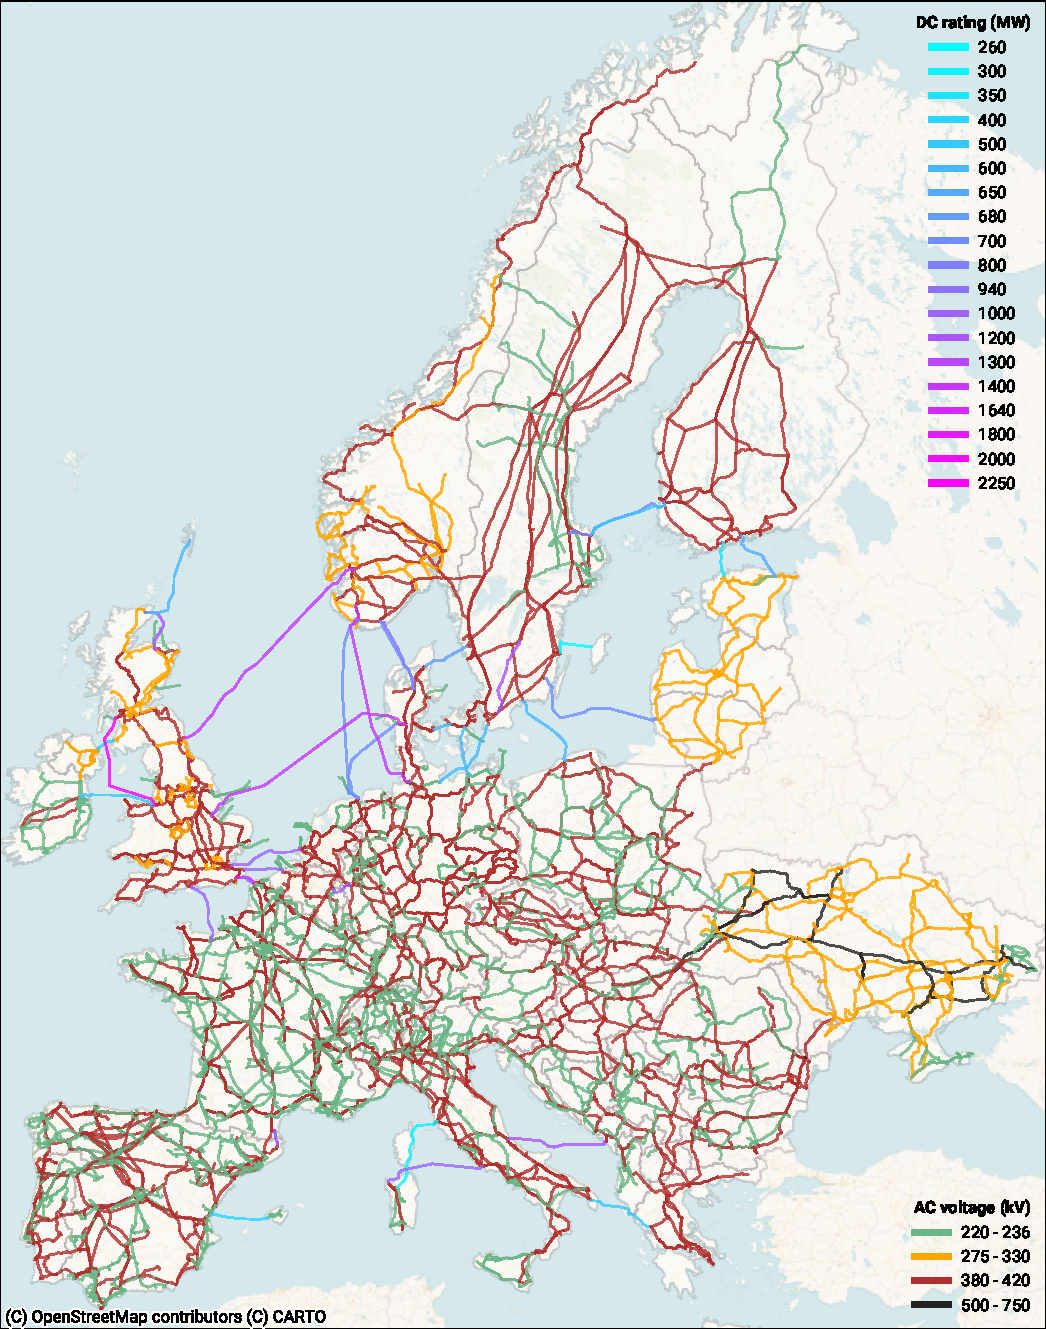
\includegraphics[width=1\textwidth]{osm_map}
    \end{column}
  \end{columns}
  \source{Own illustration based on data extracted using Overpass Turbo API\\\url{https://openstreetmap.org}}
  
  
\end{frame}

\end{document}